%==============================================================================
% MAT3300 Mathematical Modeling — Final Project Report Template (single file)
% Problem C: 2021 ICM Problem D — The Influence of Music
%
% Structure per Final_Project_Guidelines.pdf and the Problem C statement:
%   1. One-page Summary Sheet  (team members' full names + student IDs at the
%      top, as required by the course guidelines)
%   2. Table of Contents
%   3. Complete solution (main body)
%   4. One-page document to the ICM Society  (value of approach, effect of
%      richer data, further study recommendations — required by Problem C)
%   5. References
%   6. Contribution statement  (EXTRA page, NOT counted in the 25-page limit)
%
% TOTAL page budget for items 1–5: at most 25 pages.
%
% Compile:  pdflatex main.tex  (run TWICE so the ToC and cross-references
%           resolve), or: latexmk -pdf main.tex
%==============================================================================
\documentclass[11pt,letterpaper]{article}

%------------------------------------------------------------------------------
% Page layout & typography
%------------------------------------------------------------------------------
\usepackage[margin=1in]{geometry}
\usepackage{microtype}
\usepackage{fancyhdr}
\usepackage{titlesec}
\usepackage{setspace}

%------------------------------------------------------------------------------
% Math
%------------------------------------------------------------------------------
\usepackage{amsmath,amssymb,amsfonts,amsthm}
\usepackage{mathtools}
\usepackage{bm}
\usepackage{siunitx}

%------------------------------------------------------------------------------
% Graphics, tables, figures
%------------------------------------------------------------------------------
\usepackage{graphicx}
\graphicspath{{./figures/}}     % put all figure files in ./figures/
\usepackage{booktabs}
\usepackage{multirow}
\usepackage{longtable}
\usepackage{tabularx}
\usepackage{threeparttable}
\usepackage{caption}
\usepackage{subcaption}
\captionsetup{font=small,labelfont=bf}

%------------------------------------------------------------------------------
% Algorithms, code listings, colors
%------------------------------------------------------------------------------
\usepackage{algorithm}
\usepackage{algpseudocode}
\usepackage{listings}
\usepackage{xcolor}
\lstset{
  language=Python, basicstyle=\ttfamily\footnotesize,
  keywordstyle=\color{blue!60!black}\bfseries,
  backgroundcolor=\color{gray!6}, frame=single, breaklines=true,
  numbers=left, numberstyle=\tiny\color{gray}
}

%------------------------------------------------------------------------------
% Diagrams (optional)
%------------------------------------------------------------------------------
\usepackage{tikz}
\usetikzlibrary{arrows.meta,positioning,shapes.geometric}

%------------------------------------------------------------------------------
% Lists, cross-references, hyperlinks (hyperref LAST, cleveref after it)
%------------------------------------------------------------------------------
\usepackage{enumitem}
\usepackage[colorlinks=true,linkcolor=blue,citecolor=blue,urlcolor=blue]{hyperref}
\usepackage{cleveref}

\numberwithin{equation}{section}

%------------------------------------------------------------------------------
% Header / footer
%------------------------------------------------------------------------------
\pagestyle{fancy}
\fancyhf{}
\fancyhead[L]{\small MAT3300 Final Project}
\fancyfoot[C]{\thepage}
\renewcommand{\headrulewidth}{0.4pt}

%==============================================================================
% Team information
%==============================================================================
\newcommand{\TeamMembers}{%
  Yu Zihan (123090773)\quad
  Qian Chenghao (123090452)\quad
  Li Peixuan (123090276)}

%==============================================================================
\begin{document}
%==============================================================================

%------------------------------------------------------------------------------
% 1. SUMMARY SHEET — one page, must stand on its own; write it LAST.
%    Cover: problem, approach, key results (with numbers), validation, conclusion.
%------------------------------------------------------------------------------
\thispagestyle{empty}
\begin{center}
  {\LARGE\bfseries Measuring Musical Influence: A Directed-Network Approach
   to the Evolution of Music}\\[10pt]
  {\normalsize \TeamMembers}\\[4pt]
  {\small MAT3300 Mathematical Modeling --- Final Project, CUHK-Shenzhen}
\end{center}
\vspace{0.8em}
\noindent\rule{\textwidth}{0.6pt}
\vspace{0.8em}
\begin{center}
  {\Large\bfseries Summary}
\end{center}
% TODO: summary text (problem -> approach -> key results -> validation -> conclusion)
\vspace{0.6em}
\noindent\textbf{Keywords:} directed network; musical influence; similarity
measurement; genre evolution; PageRank; sensitivity analysis
\newpage

%------------------------------------------------------------------------------
% 2. TABLE OF CONTENTS
%------------------------------------------------------------------------------
\tableofcontents
\newpage

%------------------------------------------------------------------------------
% 3. COMPLETE SOLUTION
%------------------------------------------------------------------------------
\pagenumbering{arabic}

\section{Introduction and Problem Restatement}\label{sec:intro}
% TODO: background; restatement of the 7 tasks from Problem C; roadmap.

\section{Assumptions and Justifications}\label{sec:assumptions}
% TODO: numbered assumptions A1, A2, ... each with a justification.

\section{Notation}\label{sec:notation}

\Cref{tab:notation} lists the symbols used throughout the report, grouped into Model~I (network), Model~II (features), Model~III (genre
flow / relatedness), and Model~IV (temporal revolutions).

\begin{table}[htbp]
\centering
\caption{Main notation. Upper block: directed influence network (Model~I).
Middle: audio features (Model~II). Lower blocks: genre flow (Model~III)
and temporal dual-channel leaps (Model~IV).}
\label{tab:notation}
\begin{tabular}{@{}ll@{}}
\toprule
\multicolumn{2}{@{}l}{\emph{Network (Model~I)}} \\
\midrule
$G=(V,E)$ & Directed influence network; $i\to j$ means ``$i$ reported as an influence on $j$'' \\
$N=|V|$   & Number of artists (nodes) \\
$A_{ij}$  & Adjacency indicator, $A_{ij}=\mathbf{1}[i\to j\in E]$ \\
$w_{ij}$  & Edge weight ($w_{ij}=1$ in Model~I) \\
$d_i^{\text{out}},\; d_i^{\text{in}}$ & Out-/in-degree of node $i$ \\
$d_j^{\leftarrow,\text{out}}$ & Out-degree of $j$ within the reversed graph $G^{\leftarrow}$ \\
$G^{\leftarrow}$ & Reversed graph in which every edge is flipped, so a follower endorses its influencer \\
$K_i$     & Outgoing Katz centrality of artist $i$ \\
$\alpha$  & Katz attenuation factor \\
$\rho$    & Spectral radius of the adjacency matrix $A$ \\
$\mathrm{PR}^{\text{rev}}_i$ & Reverse PageRank of artist $i$ (computed on $G^{\leftarrow}$) \\
$\delta$  & PageRank damping factor ($\delta=0.85$) \\
$C_d$     & Cohort of followers whose active-start decade is $d$ \\
$G_S$     & Genre-induced subnetwork over artists of genre $S$ \\
\midrule
\multicolumn{2}{@{}l}{\emph{Audio features (Model~II)}} \\
\midrule
$\mathbf{x}_i\in\mathbb{R}^{p}$ & Artist $i$'s Spotify feature vector \\
$\tilde{\mathbf{x}}_i$ & $z$-score standardized feature vector \\
$p$ & Number of audio features ($p=11$ in our baseline) \\
$d_{ij}=\|\tilde{\mathbf{x}}_i-\tilde{\mathbf{x}}_j\|_2$ & Euclidean distance (dissimilarity) \\
$\mathcal{G}(i)$ & Main genre label of artist $i$ \\
$W$, $B$ & Sets of within-genre / between-genre artist pairs \\
$\bar{d}_{\mathrm{within}}$, $\bar{d}_{\mathrm{between}}$ & Mean distances over $W$ and $B$ \\
$r$ & Number of retained PCA components \\
\midrule
\multicolumn{2}{@{}l}{\emph{Genre flow / relatedness (Model~III)}} \\
\midrule
$F(t)$ & Genre-to-genre influence-edge count matrix for followers starting in decade $t$ \\
$c_{\mathrm{cross}}(t)$ & Cross-genre share of $F(t)$ \\
$c_K(t)$ & Katz-weighted cross-genre share of influence in decade $t$ \\
$K_g(t)$ & Genre share of outgoing Katz mass among artists starting in decade $t$ \\
$c_g$ & Katz-weighted genre centroid in feature space (Model~III similarity) \\
\midrule
\multicolumn{2}{@{}l}{\emph{Temporal dual-channel (Model~IV / Task~5)}} \\
\midrule
$\mathbf{x}(t)$ & Year-$t$ $z$-scored industry feature state from \texttt{data\_by\_year} \\
$E(t)$ & Sonic leap size $\|\mathbf{x}(t)-\mathbf{x}(t-1)\|_2$ \\
$N(t)$ & Network-restructuring score from $\Delta c_{\mathrm{cross}}$, $\Delta c_K$, and Katz-mass turnover \\
$\tau(t)$ & $\ell_1$ turnover of genre shares of outgoing Katz mass $K_g(t)$ \\
\bottomrule
\end{tabular}
\end{table}


\section{Data Preprocessing and Exploration}\label{sec:data}

We use only the official files in \texttt{ProblemC\_Music\_data/}; no
external data are introduced. Of the four files,
\texttt{influence\_data.csv} ($42{,}770$ directed influencer$\to$follower
edges, with both artists' \texttt{main\_genre} and \texttt{active\_start}
decade) is the primary input to Model~I and also serves as the genre
dictionary for Model~II, and \texttt{data\_by\_artist.csv} ($5{,}810$
artists) provides artist-level mean Spotify features for Model~II; the
song-level \texttt{full\_music\_data.csv} and yearly
\texttt{data\_by\_year.csv} are reserved for finer temporal analyses and
are not used in the models below. This section documents the two cleaning
pipelines and two data-quality audits whose findings shape every later
model; the influence data require their own cleaning, and the feature
data a different one, so we keep the two pipelines explicit and separate.

\subsection{Cleaning of the Influence Data}\label{subsec:data-cleaning}

The raw influence file requires four repairs before it can be used.
(i)~\emph{Identifier hygiene}: trailing whitespace in artist identifiers and
names is trimmed. (ii)~\emph{Encoding artefacts}: mojibake in some artist
names is repaired by re-decoding the affected strings. (iii)~\emph{Label
repair}: genre labels contain an HTML-escape residue (e.g.\ ``R\&B;''
$\to$ ``R\&B''), which we strip. (iv)~\emph{Type coercion}: active-start
fields are cast to decade integers. After these repairs we check for
duplicated directed pairs; none exist, so all 42{,}770 unique directed pairs
are retained, spanning $N=5{,}603$ artists.

\subsection{Cleaning Choices for Model~II}\label{subsec:data-cleaning-features}

\begin{enumerate}
  \item Join \texttt{data\_by\_artist} to genre labels via
        \texttt{artist\_id}, where genres are taken from
        \texttt{influence\_data} (we do \emph{not} redefine Pop/Rock or
        other genres; see Assumption~A4).
  \item Drop artists with missing genre or genre \texttt{Unknown}.
  \item Select $p=11$ numeric features: danceability, energy, valence,
        tempo, loudness, acousticness, instrumentalness, liveness,
        speechiness, duration\_ms, popularity.
  \item Apply column-wise $z$-score standardization before computing
        Euclidean distances (see Model~II). We note that
        \emph{popularity} is not comparable across eras---it rises almost
        monotonically from 1921 to 2020 in \texttt{data\_by\_year}---so a
        within-year normalization variant is examined as a robustness check
        in Model~II.
\end{enumerate}
After cleaning we retain $n=5{,}599$ artists with both features and a genre
label, covering 19 genres (Pop/Rock is the largest class). This similarity
sample ($5{,}599$ artists) is not identical to the network sample
($5{,}603$ artists of \cref{subsec:data-cleaning}); the small discrepancy
arises because having a genre label, having Spotify features, and appearing
in the influence data are three separate conditions, and any analysis that
crosses the two samples uses their intersection (stated explicitly where it
occurs).

\subsection{Data-Quality Audit}\label{subsec:data-audit}

Two structural facts of the influence data shape every later model, so we
audit them here rather than inside any single model.

\emph{Time-order consistency.} Decade information allows a consistency
check that the raw data never advertises: in 733 edges (1.7\%) the
follower's active-start decade precedes the influencer's, and in 8{,}477
edges the two decades coincide. Per Assumption~A3 the 733 reversals are
retained in the primary network and their effect is quantified in
\cref{subsec:q1-robustness}; same-decade edges are kept as same-generation
mutual influence.

\emph{Skewed connectivity and genre concentration.} The out-degree
distribution is heavily right-skewed (mean 11.3, median 5, maximum 615 for
The Beatles), while in-degrees are moderate (median 7, maximum 47): being
cited is bounded by list length, citing is not. Genre labels concentrate
sharply---Pop/Rock accounts for 56\% of all edges---and 76.6\% of edges
connect same-genre artists. These facts motivate the log-scale treatment of
degree in \cref{subsec:q1-global}, the cohort view of
\cref{subsec:q1-cohorts}, and the genre-comparison design of Model~III.



\section{Model I: Directed Influence Network}\label{sec:model-influence}

This section addresses Task~1: we build the reported musical-influence network,
develop parameters that capture influence, and describe the resulting structure
both globally and through two complementary lenses (temporal cohorts and a
genre-induced subnetwork).

\subsection{Network Construction}\label{subsec:net-construction}

Using the cleaned edge table of \cref{subsec:data-cleaning}, we model the
influence system as a directed graph \(G=(V,E)\), where each node
\(v\in V\) is an artist (\(|V|=5{,}603\)) and each edge \(i\to j\in E\)
records that the data report artist \(i\) as an influence on artist \(j\)
(\(|E|=42{,}770\)). Because the data record the \emph{existence} of a
reported relation rather than its strength, we assign every edge the
baseline weight \(w_{ij}=1\) (Assumption~A1); constructing edge strengths
from musical evidence is deferred to Model~II. Genre and active-start
decade are attached to nodes as descriptive attributes (Assumption~A2),
and the 733 time-order-reversed edges identified in the data audit are
retained in the primary network (Assumption~A3), with their effect
quantified separately in \cref{subsec:q1-robustness}.

\subsection{Influence Measures and Network Topology}\label{subsec:q1-measures}

We report three measures with deliberately distinct interpretations rather
than a single weighted composite: each answers a different question, and their
agreement (or disagreement) is itself informative.

\paragraph{Out-degree.}
The number of artists who directly name \(i\) as an influence,
\begin{equation}
d_i^{\text{out}}=\sum_{j} A_{ij}, \qquad A_{ij}=\mathbf{1}[i\to j\in E],
\end{equation}
measures \emph{direct} reach. It is transparent but blind to indirect
transmission.

\paragraph{Outgoing Katz centrality (primary measure).}
To capture multi-step influence we use Katz centrality computed on outgoing
paths,
\begin{equation}\label{eq:katz}
K_i=\Bigl[(I-\alpha A)^{-1}\mathbf{1}\Bigr]_i
   =1+\alpha (A\mathbf{1})_i+\alpha^2(A^2\mathbf{1})_i+\cdots,
\end{equation}
which counts all directed walks leaving \(i\), each additional hop discounted
by the attenuation factor \(\alpha\in(0,1/\rho)\), where \(\rho\) is the
spectral radius of \(A\). For our network \(\rho=3.614\), so
\(\alpha<0.2767\) guarantees convergence; we use \(\alpha=0.10\), which keeps
a comfortable margin from the bound while weighting second- and third-step
transmission substantially (a path of length \(\ell\) contributes
\(\alpha^{\ell-1}\)). Intuitively, \(K_i\) rewards artists whose followers
themselves went on to influence many others: influencing one future
``hub'' can be worth more than influencing many dead-end artists.

\paragraph{Reverse PageRank (comparison measure).}
PageRank scores a node by the PageRank of the nodes that point to it. On the
raw edge direction, that would measure \emph{receiving} influence. We therefore
compute PageRank on the reversed graph \(G^{\leftarrow}\), in which every edge
is flipped so that a follower endorses its influencer:
\begin{equation}\label{eq:rpr}
\mathrm{PR}^{\text{rev}}_i=\frac{1-\delta}{N}
 +\delta\sum_{j\to i\,\in\,G^{\leftarrow}}\frac{\mathrm{PR}^{\text{rev}}_j}{d_j^{\leftarrow,\text{out}}},
 \qquad \delta=0.85,
\end{equation}
where \(d_j^{\leftarrow,\text{out}}\) is \(j\)'s out-degree within the
reversed graph (equivalently, its in-degree in \(G\)), so that recognition
flows from reported followers back to the artists they credit. We state
this reversal explicitly because it is the difference between
``being shaped by important artists'' and ``shaping important artists''.

We do \emph{not} merge the three measures into an ad hoc weighted index:
they encode different semantics, and any fixed weighting would be
arbitrary; instead we compare their rankings, and
\cref{subsec:q1-robustness} shows the conclusions are robust to this
choice.

\Cref{tab:q1-topology} summarises the network. The graph is almost fully
connected in the weak sense (99.9\% of artists lie in one weak component),
but fragmented into many strong components: influence, as reported, flows
through a giant downstream cascade rather than forming tightly reciprocated
clusters. The 1{,}829 artists with zero out-degree have no recorded
followers in this dataset---a statement about the data, not proof of
absence of influence; the decade lag between influencer and follower is
consistent with the one-to-two-generation transmission delay expected of
influence.

\begin{table}[htbp]
\centering
\caption{Topology of the reported influence network.}
\label{tab:q1-topology}
\begin{tabular}{lr}
\toprule
Statistic & Value \\
\midrule
Reported pairs (unique directed edges) & 42{,}770 \\
Artists (nodes) & 5{,}603 \\
Weakly connected components & 3 \\
Largest weak component & 5{,}599 (99.9\%) \\
Strongly connected components & 4{,}747 \\
Largest strong component & 778 \\
Artists with zero out-degree & 1{,}829 \\
Artists with zero in-degree & 557 \\
Edges with reversed decade order (retained) & 733 (1.7\%) \\
Edges with same-decade endpoints & 8{,}477 \\
\bottomrule
\end{tabular}
\end{table}

\subsection{Global Results: Leading Influencers}\label{subsec:q1-global}

\Cref{fig:q1-global} presents the primary results. The Katz ranking is led by
Chuck Berry, followed by The Beatles, Muddy Waters, Louis Jordan and Bob
Dylan (\cref{tab:q1-top10}). The contrast between the two panels of
\cref{fig:q1-global} is the central empirical finding of this section:
\emph{direct} and \emph{multi-step} influence agree in bulk
(Spearman \(\rho=0.953\) overall) yet diverge sharply at the top. The Beatles
hold by far the largest direct following (out-degree 615), but Chuck Berry---
with only 159 direct followers---outranks them in Katz terms because his
followers include artists who themselves became massive transmission hubs.
Multi-step credit, in other words, rewards artists whose influence
\emph{propagates} through the network, not merely those who accumulate the
most direct citations. Muddy Waters, Louis Jordan, Hank Williams and Howlin'
Wolf illustrate the same mechanism from older generations: modest direct
lists, but followers who carried blues and jazz idioms into the rock era.

\begin{table}[htbp]
\centering
\caption{Top-10 artists by outgoing Katz centrality (\(\alpha=0.10\)),
with direct out-degree and rank under reverse PageRank for comparison.}
\label{tab:q1-top10}
\begin{tabular}{rlrrr}
\toprule
Rank & Artist & \(K_i\) & \(d_i^{\text{out}}\) & PR\(^{\text{rev}}\) rank \\
\midrule
1 & Chuck Berry      & 713.4 & 159 & 19 \\
2 & The Beatles      & 691.8 & 615 & 7  \\
3 & Muddy Waters     & 580.0 & 113 & 13 \\
4 & Louis Jordan     & 549.5 & 53  & 4  \\
5 & Bob Dylan        & 545.3 & 389 & 14 \\
6 & Hank Williams    & 543.6 & 184 & 18 \\
7 & Little Richard   & 537.6 & 88  & 26 \\
8 & Elvis Presley    & 515.2 & 166 & 27 \\
9 & Roy Brown        & 513.2 & 34  & 25 \\
10 & Howlin' Wolf    & 435.9 & 99  & 29 \\
\bottomrule
\end{tabular}
\end{table}

\begin{figure}[htbp]
\centering
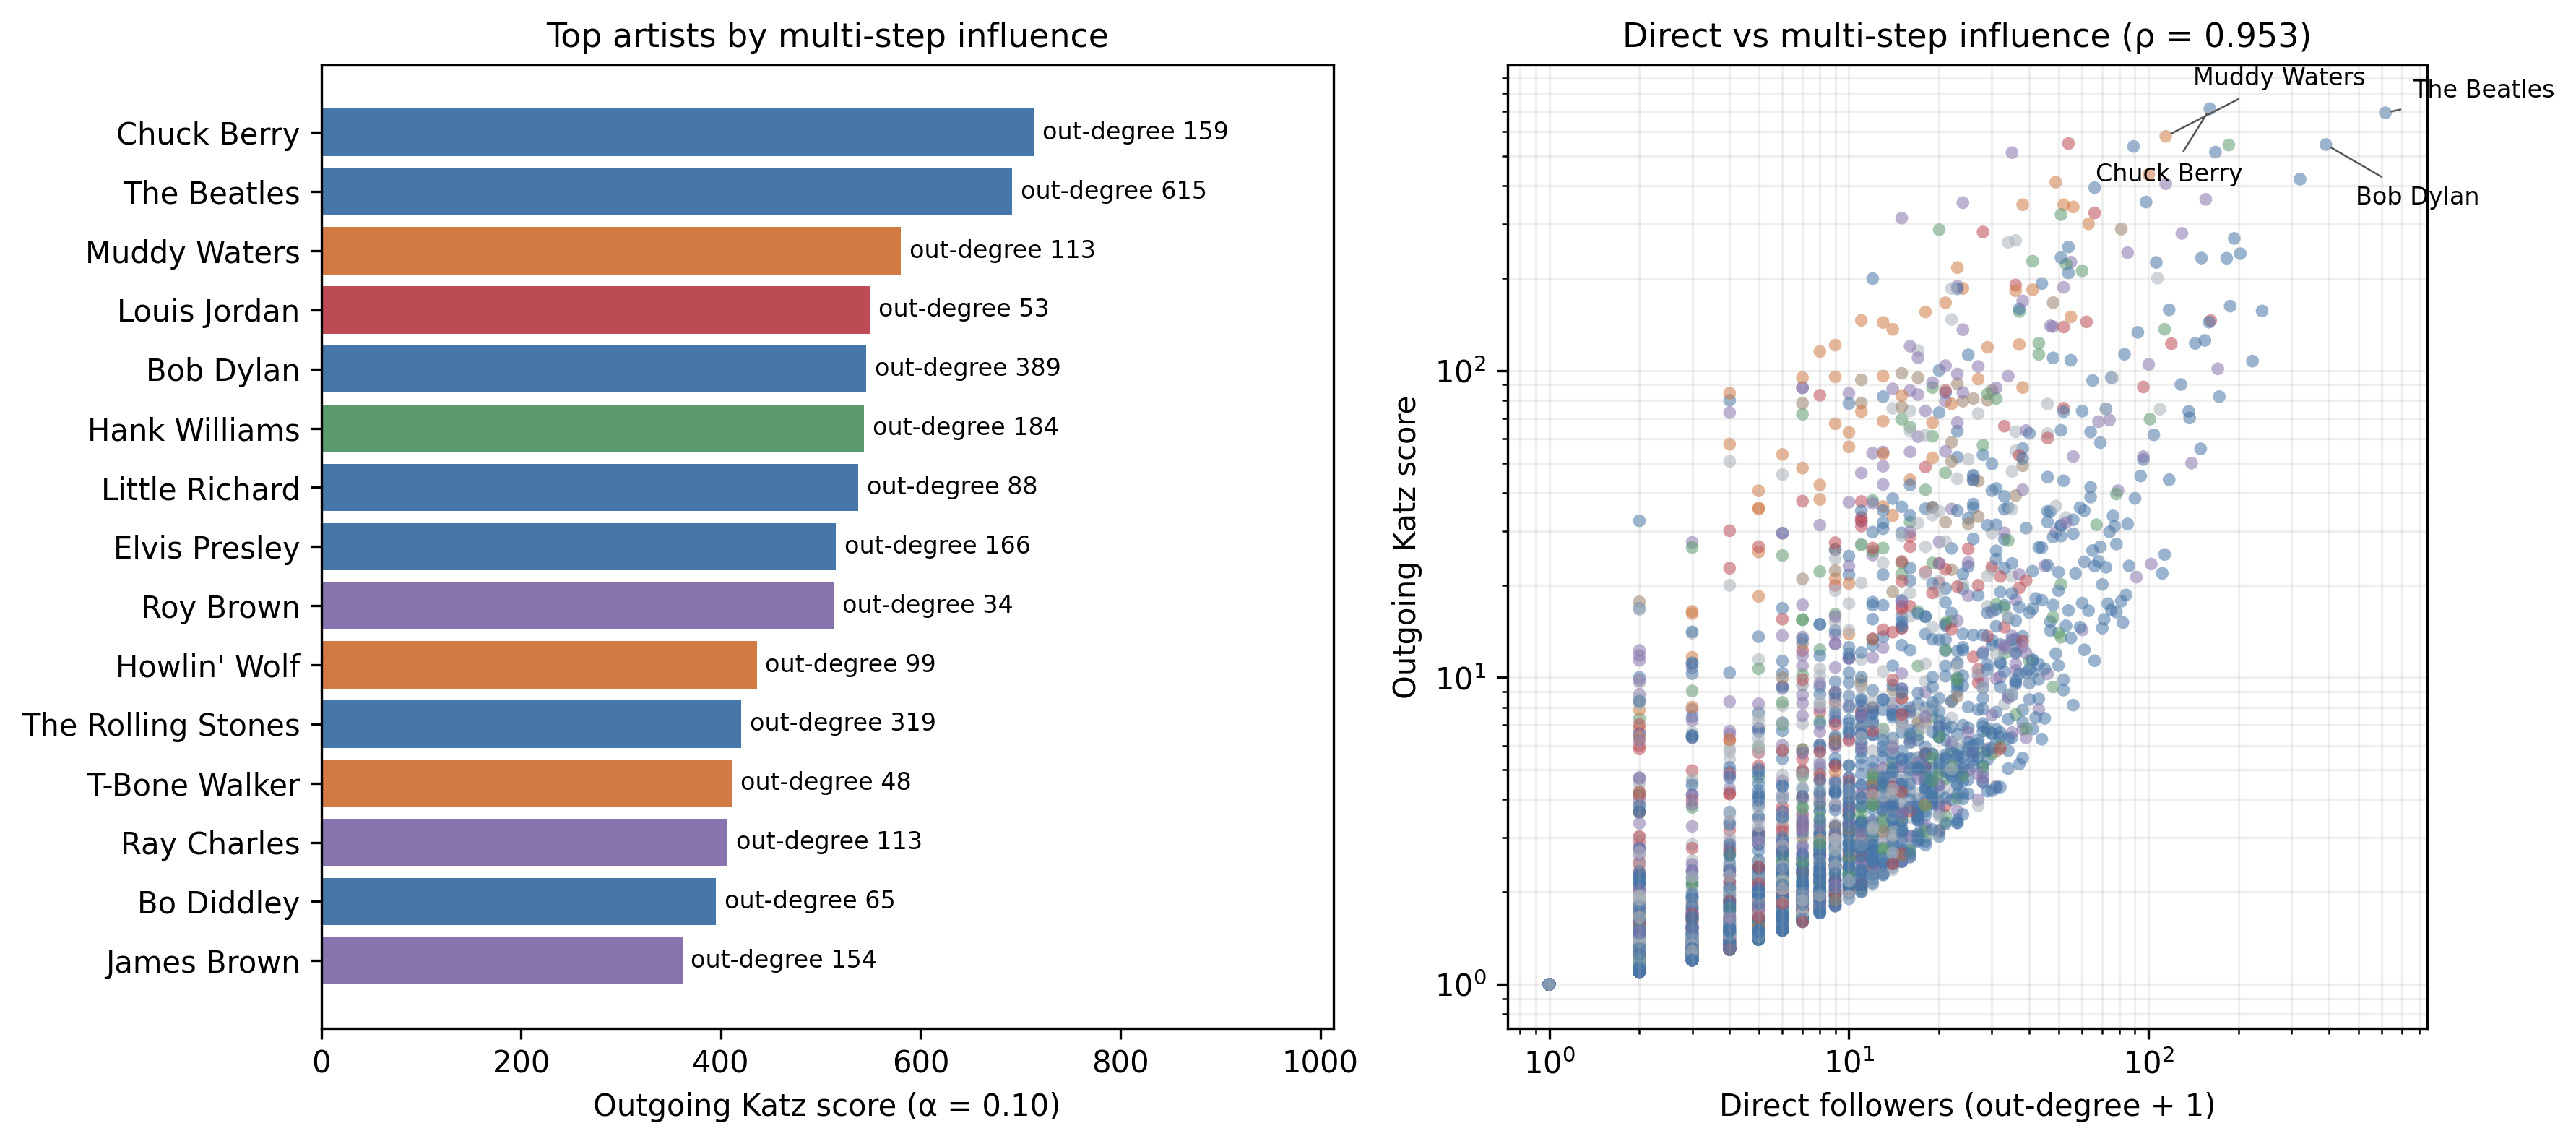
\includegraphics[width=\textwidth]{fig1_global_influence.png}
\caption{Global influence rankings. \emph{Left:} top-15 artists by outgoing
Katz score (\(\alpha=0.10\)); bar colour encodes the artist's main genre and
the annotation gives the raw out-degree. \emph{Right:} direct followers
(out-degree) versus Katz score on log--log axes; artists far above the
diagonal owe their position to indirect, multi-step transmission
(Spearman \(\rho=0.953\)).}
\label{fig:q1-global}
\end{figure}

The reverse-PageRank column of \cref{tab:q1-top10} reveals a systematic
difference in character: its global top ranks are occupied by early-era
artists (Cab Calloway, Billie Holiday and Lester Young lead the overall
ranking), because under recursive endorsement an artist active in the
1930s has had nine decades to accumulate credit. This is the well-known
age bias of centrality measures on growing networks: reverse PageRank
measures \emph{accumulated recognition}, while outgoing Katz measures
\emph{transmission capacity}. We report both and treat the divergence as
informative rather than averaging it away; an era-normalised variant is
discussed as a refinement in \cref{sec:validation}.

\subsection{A Dynamic View: Follower-Start-Decade Cohorts}\label{subsec:q1-cohorts}

To expose the temporal structure of reported influence without claiming exact
influence dates (Assumption~A2), we group all edges by the follower's
active-start decade and recompute the network and Katz scores within each
\emph{follower-start-decade cohort} \(C_d\). A cohort answers the question
``which influencers are credited by the artists who \emph{began} in decade
\(d\)?''---it does not date when the influence happened.

\Cref{fig:q1-cohorts} tracks the 15 artists who most often rank in a cohort's
top 10, and \cref{tab:q1-cohorts} lists cohort sizes and leading names. Three
patterns emerge. First, \emph{generational succession}: swing-era figures
dominate the 1930s--1940s cohorts, the 1950s cohort pivots to country and
early rock, and rock artists take over from the 1960s onward. Second,
\emph{cross-generational persistence}: The Beatles rank inside the top two
of five consecutive cohorts (1960s--2000s), and Bob Dylan never leaves the
top 10 from the 1960s cohort onward. Third, \emph{cohort-specific
arrivals}: Nirvana appears only from the 1990s cohort (rank~1) and David
Bowie peaks in the 1970s--1980s---each cohort reports the canon available
to it. The 2010s cohort is much smaller (811 edges) and its top-10
membership should be read with this sample-size caveat.

\begin{figure}[htbp]
\centering
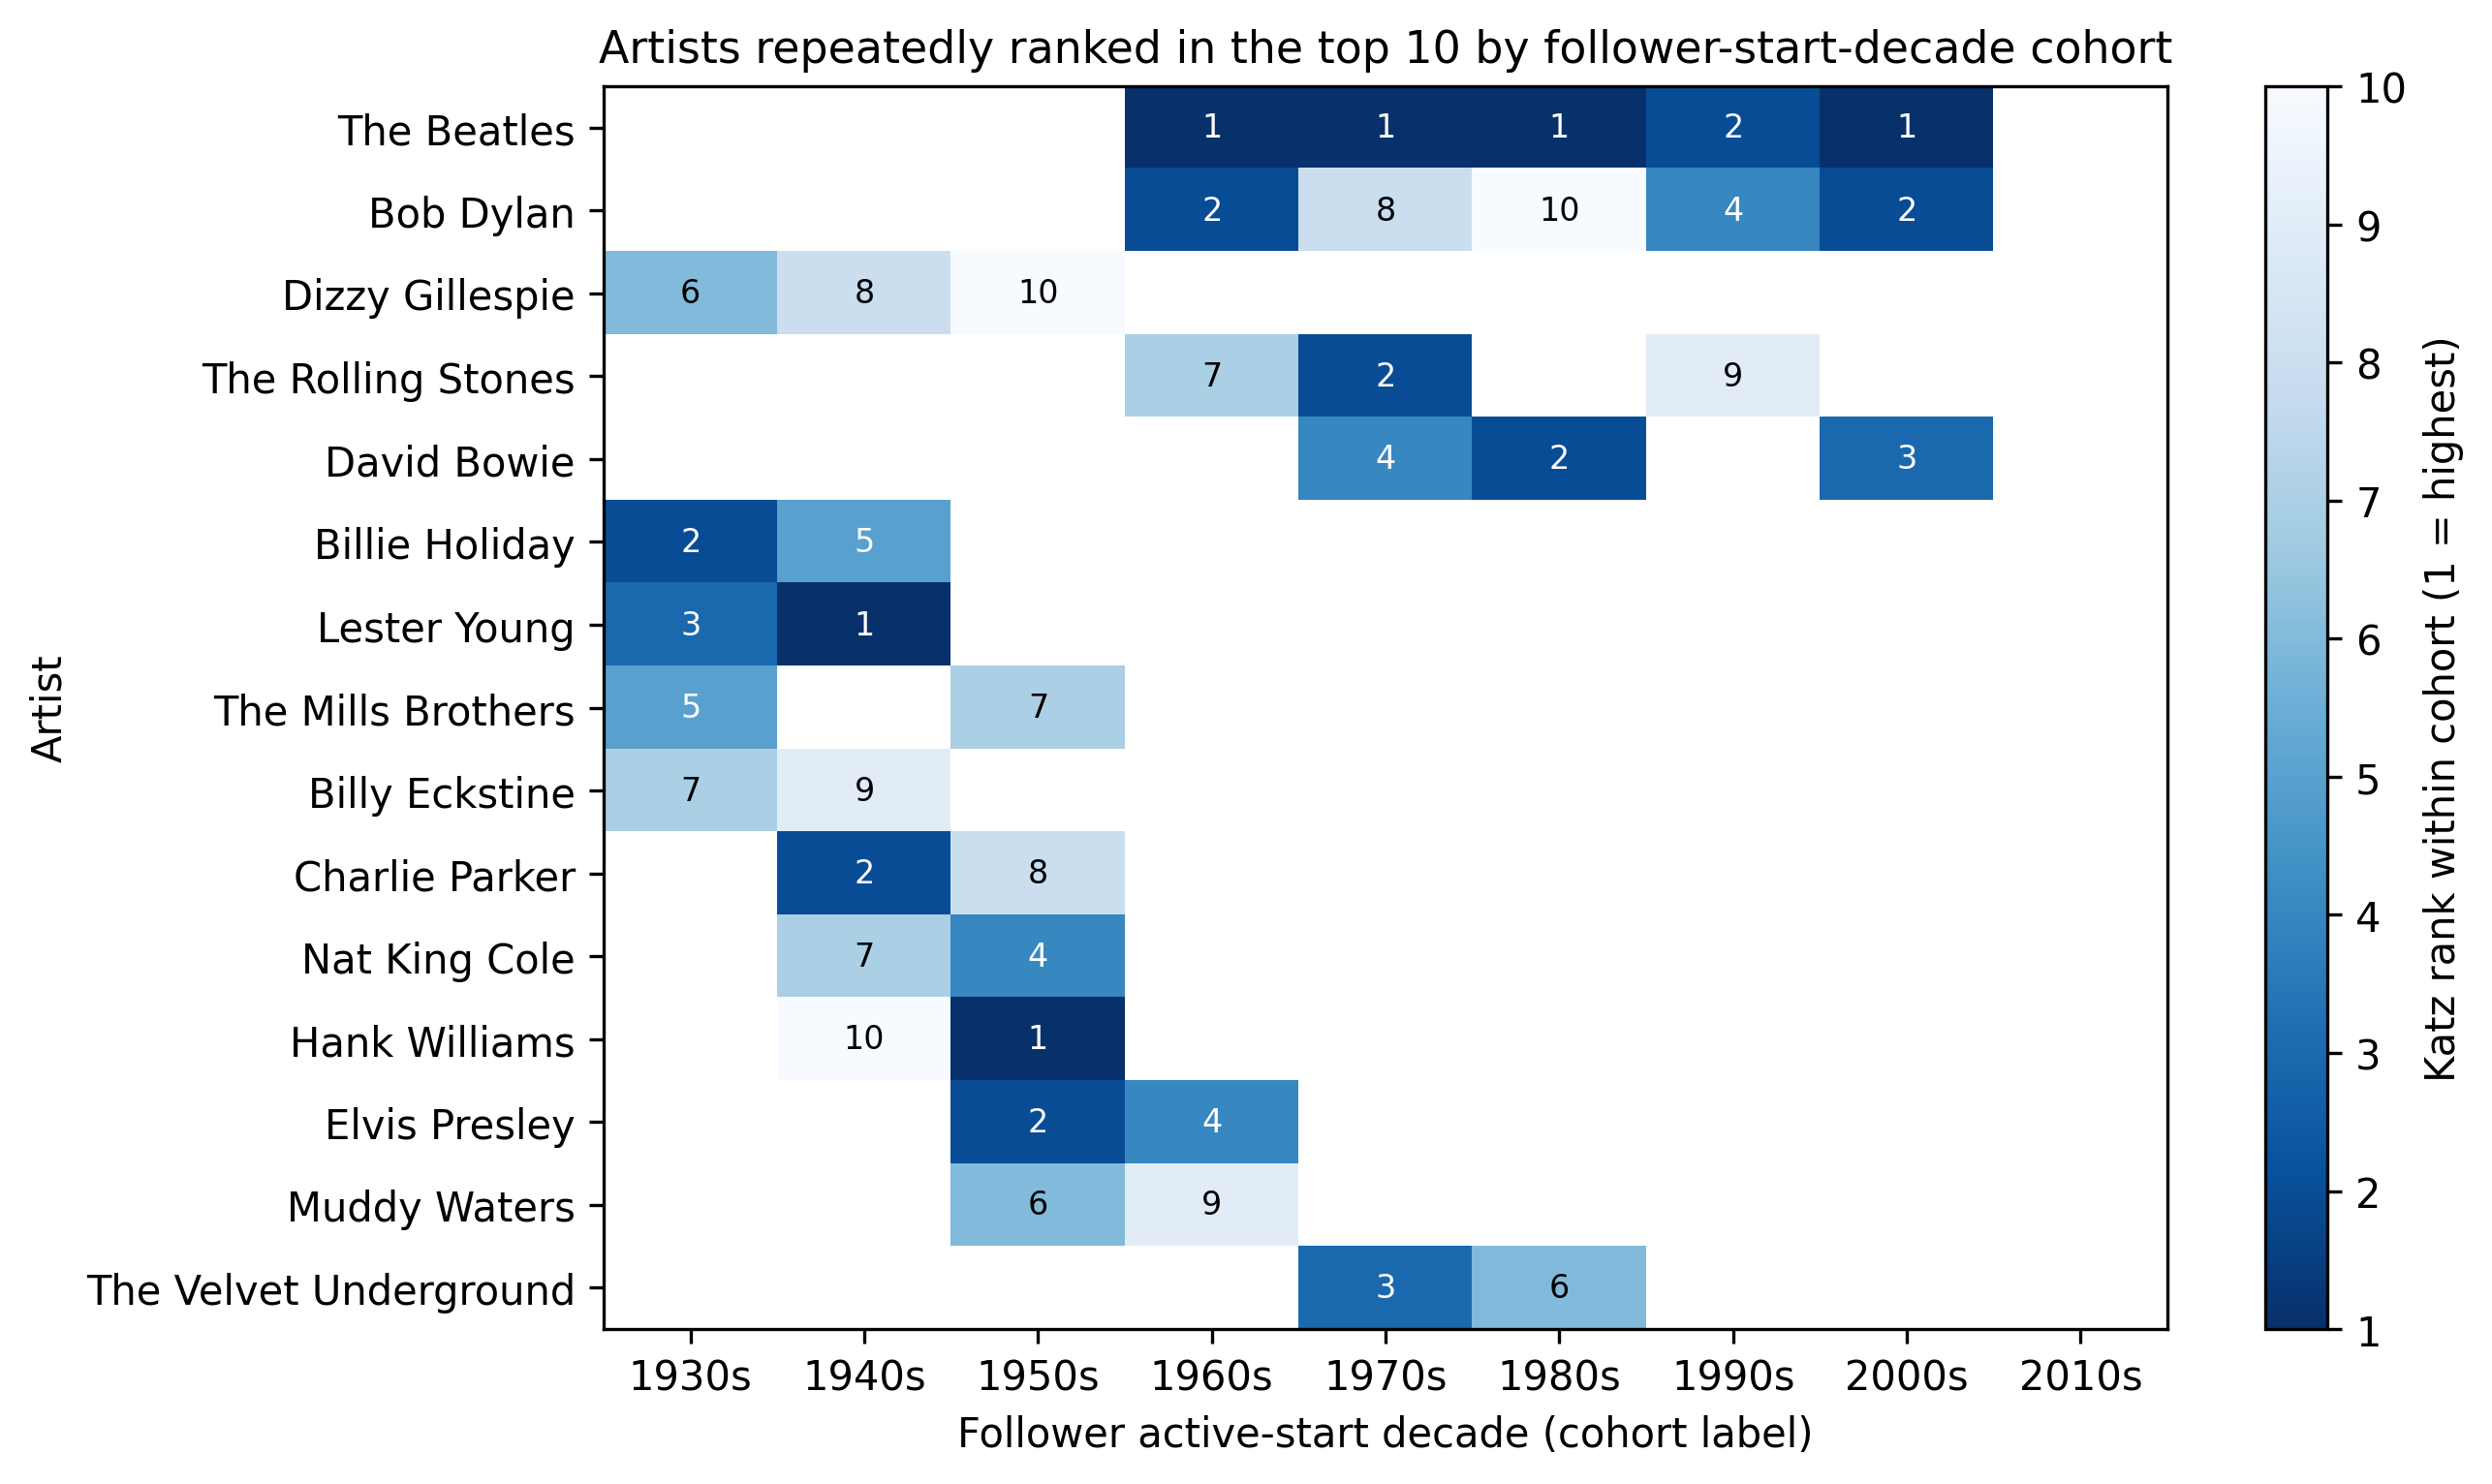
\includegraphics[width=0.92\textwidth]{fig3_cohort_heatmap.png}
\caption{Artists repeatedly ranked in the top 10 within
follower-start-decade cohorts. Each cell gives the artist's Katz rank inside
the cohort of followers who began in that decade (1 = highest; white = not in
the cohort's top 10). Cohorts group by followers' active-start decade, not by
the date an influence occurred; the 2010s cohort is small (811 edges) and its
column is correspondingly sparse.}
\label{fig:q1-cohorts}
\end{figure}

\begin{table}[htbp]
\centering
\caption{Follower-start-decade cohorts: size and three highest-scoring
influencers within each cohort (\(\alpha=0.10\)).}
\label{tab:q1-cohorts}
\begin{tabular}{lrrl}
\toprule
Cohort & Edges & Artists & Top-3 influencers within cohort \\
\midrule
1930s & 193   & 151  & Cab Calloway, Billie Holiday, Lester Young \\
1940s & 741   & 371  & Lester Young, Charlie Parker, Roy Acuff \\
1950s & 2{,}860  & 903  & Hank Williams, Elvis Presley, Ray Charles \\
1960s & 6{,}478  & 1{,}475 & The Beatles, Bob Dylan, Chuck Berry \\
1970s & 6{,}781  & 1{,}878 & The Beatles, The Rolling Stones, The Velvet Underground \\
1980s & 8{,}523  & 2{,}336 & The Beatles, David Bowie, Black Sabbath \\
1990s & 10{,}911 & 2{,}996 & Nirvana, The Beatles, Neil Young \\
2000s & 5{,}472  & 2{,}393 & The Beatles, Bob Dylan, David Bowie \\
2010s & 811   & 690  & Usher, Michael Jackson, Rihanna \\
\bottomrule
\end{tabular}
\end{table}

\subsection{A Genre-Induced Subnetwork: Jazz}\label{subsec:q1-jazz}

Task~1 also asks for a description of a subnetwork; we induce one by
keeping only edges whose \emph{both} endpoints are Jazz, yielding
$G_{\text{Jazz}}$ with 384 artists and 1{,}769 edges (density 0.012),
fragmented into 353 strong components. Jazz is a convenient slice---large
enough to be structurally informative, spanning nine decades, with a
well-documented internal history (swing $\to$ bebop $\to$ cool/hard bop
$\to$ fusion) that gives an external check on the model's ordering. The
leader by within-genre Katz is Charlie Parker (78 direct Jazz followers),
ahead of Lester Young and Miles Davis (83): the depth-over-breadth
mechanism of \cref{subsec:q1-global} recurs inside a single genre, and the
generational reading of \cref{fig:q1-jazz} (swing-era hubs feeding bebop-era
hubs, who feed later artists) mirrors the documented stylistic succession.
The subnetwork also \emph{exports} influence heavily: 409 further edges run
from Jazz artists to Pop/Rock artists, a cross-validation anchor we use in
\cref{subsec:q3-inf-time}. This same subnetwork is revisited in
\cref{sec:model-temporal} as the case study for Task~6.

\begin{figure}[htbp]
\centering
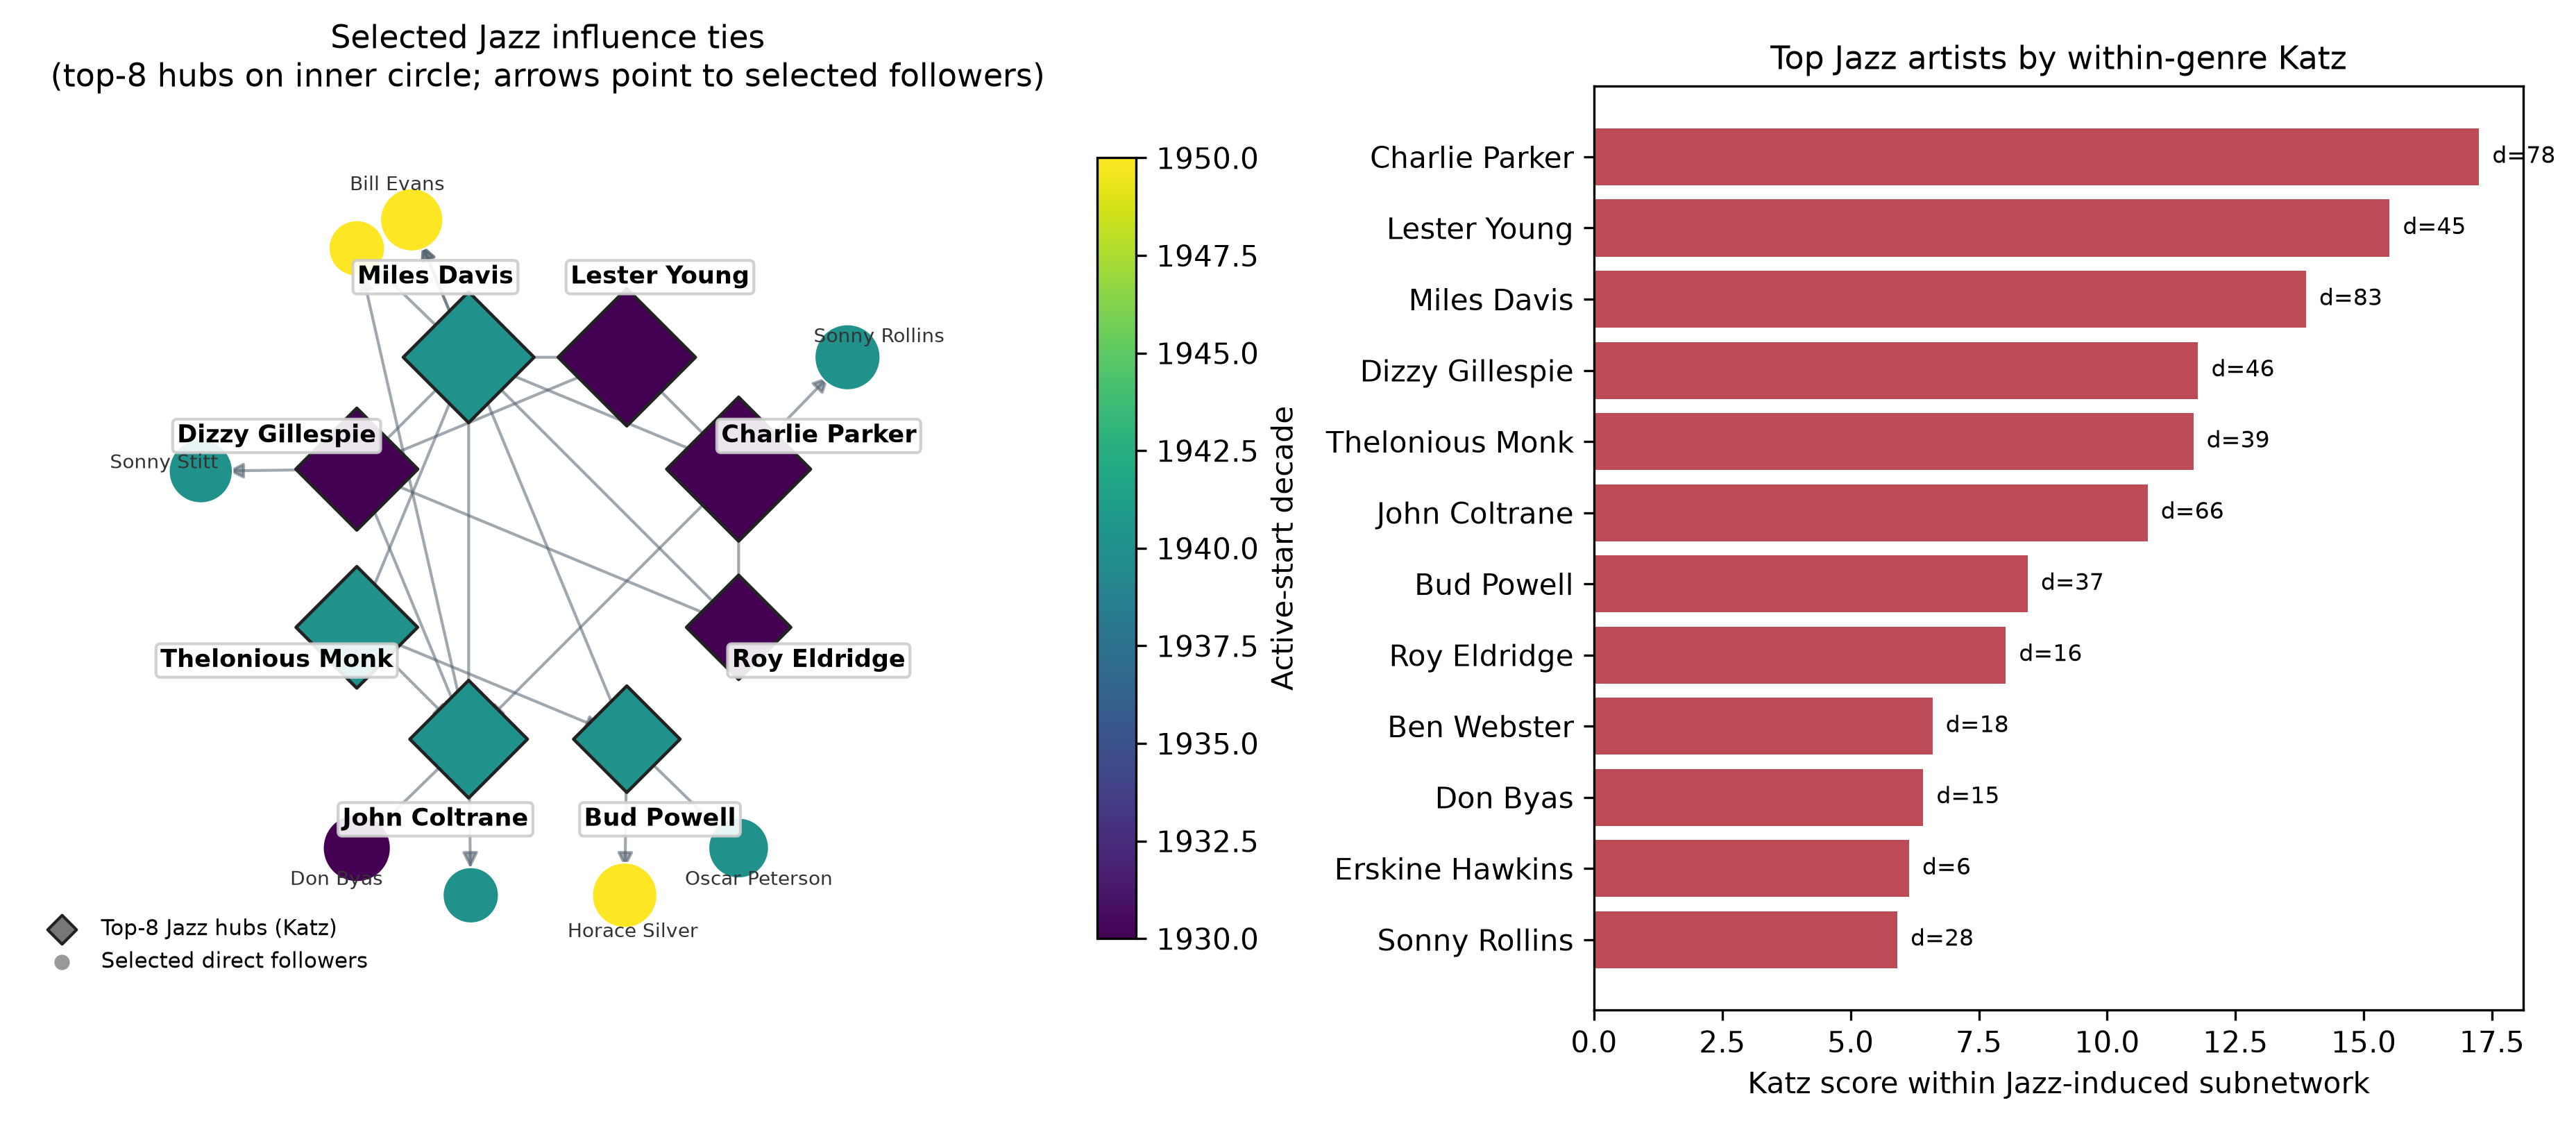
\includegraphics[width=\textwidth]{fig4_jazz_subnetwork.png}
\caption{The Jazz-induced subnetwork. \emph{Left:} selected ego view of the
top-8 Jazz hubs (diamonds, inner circle) and up to three high-scoring direct
followers each (circles, outer rays); arrow direction follows the reported
influence; colour encodes active-start decade and size the within-genre
Katz score. \emph{Right:} top-12 Jazz artists by within-genre outgoing Katz
(\(\alpha=0.10\)); annotations give direct Jazz followers \(d\).}
\label{fig:q1-jazz}
\end{figure}

\subsection{Robustness of the Rankings}\label{subsec:q1-robustness}

\Cref{fig:q1-sensitivity} verifies that the reported rankings do not depend
on analyst choices. \emph{Parameter sensitivity:} recomputing Katz over
\(\alpha\in[0.02,\,0.25]\) (the convergence bound is 0.2767), the bulk
ranking is stable---Spearman correlation with the baseline \(\alpha=0.10\)
never falls below 0.975---and the top-20 overlap is maximised exactly at the
operating point (\(20/20\) at \(\alpha=0.10\); \(16\)--\(20\) for
\(\alpha\in[0.075,0.125]\)), declining toward the extremes of the sweep
(\(9/20\) at \(\alpha=0.02\), \(8/20\) at \(\alpha=0.25\)). The extremes are
semantically degenerate rather than alarming: as \(\alpha\to0\) Katz
collapses toward raw out-degree, and as \(\alpha\) approaches the
convergence bound indirect terms dominate, so divergence there merely
reflects the intended behavioural differences. The choice
\(\alpha=0.10\) sits at the peak of both curves, comfortably inside the
stable interior. \emph{Time-filter sensitivity:} removing all 733
reversed-decade-order edges changes the Katz scores only marginally
(\(\rho=0.986\) against the primary network) and the top-20 sets are
identical (20/20 overlap). We therefore retain all reported edges in the
primary model, as stated in \cref{subsec:net-construction}.

\begin{figure}[htbp]
\centering
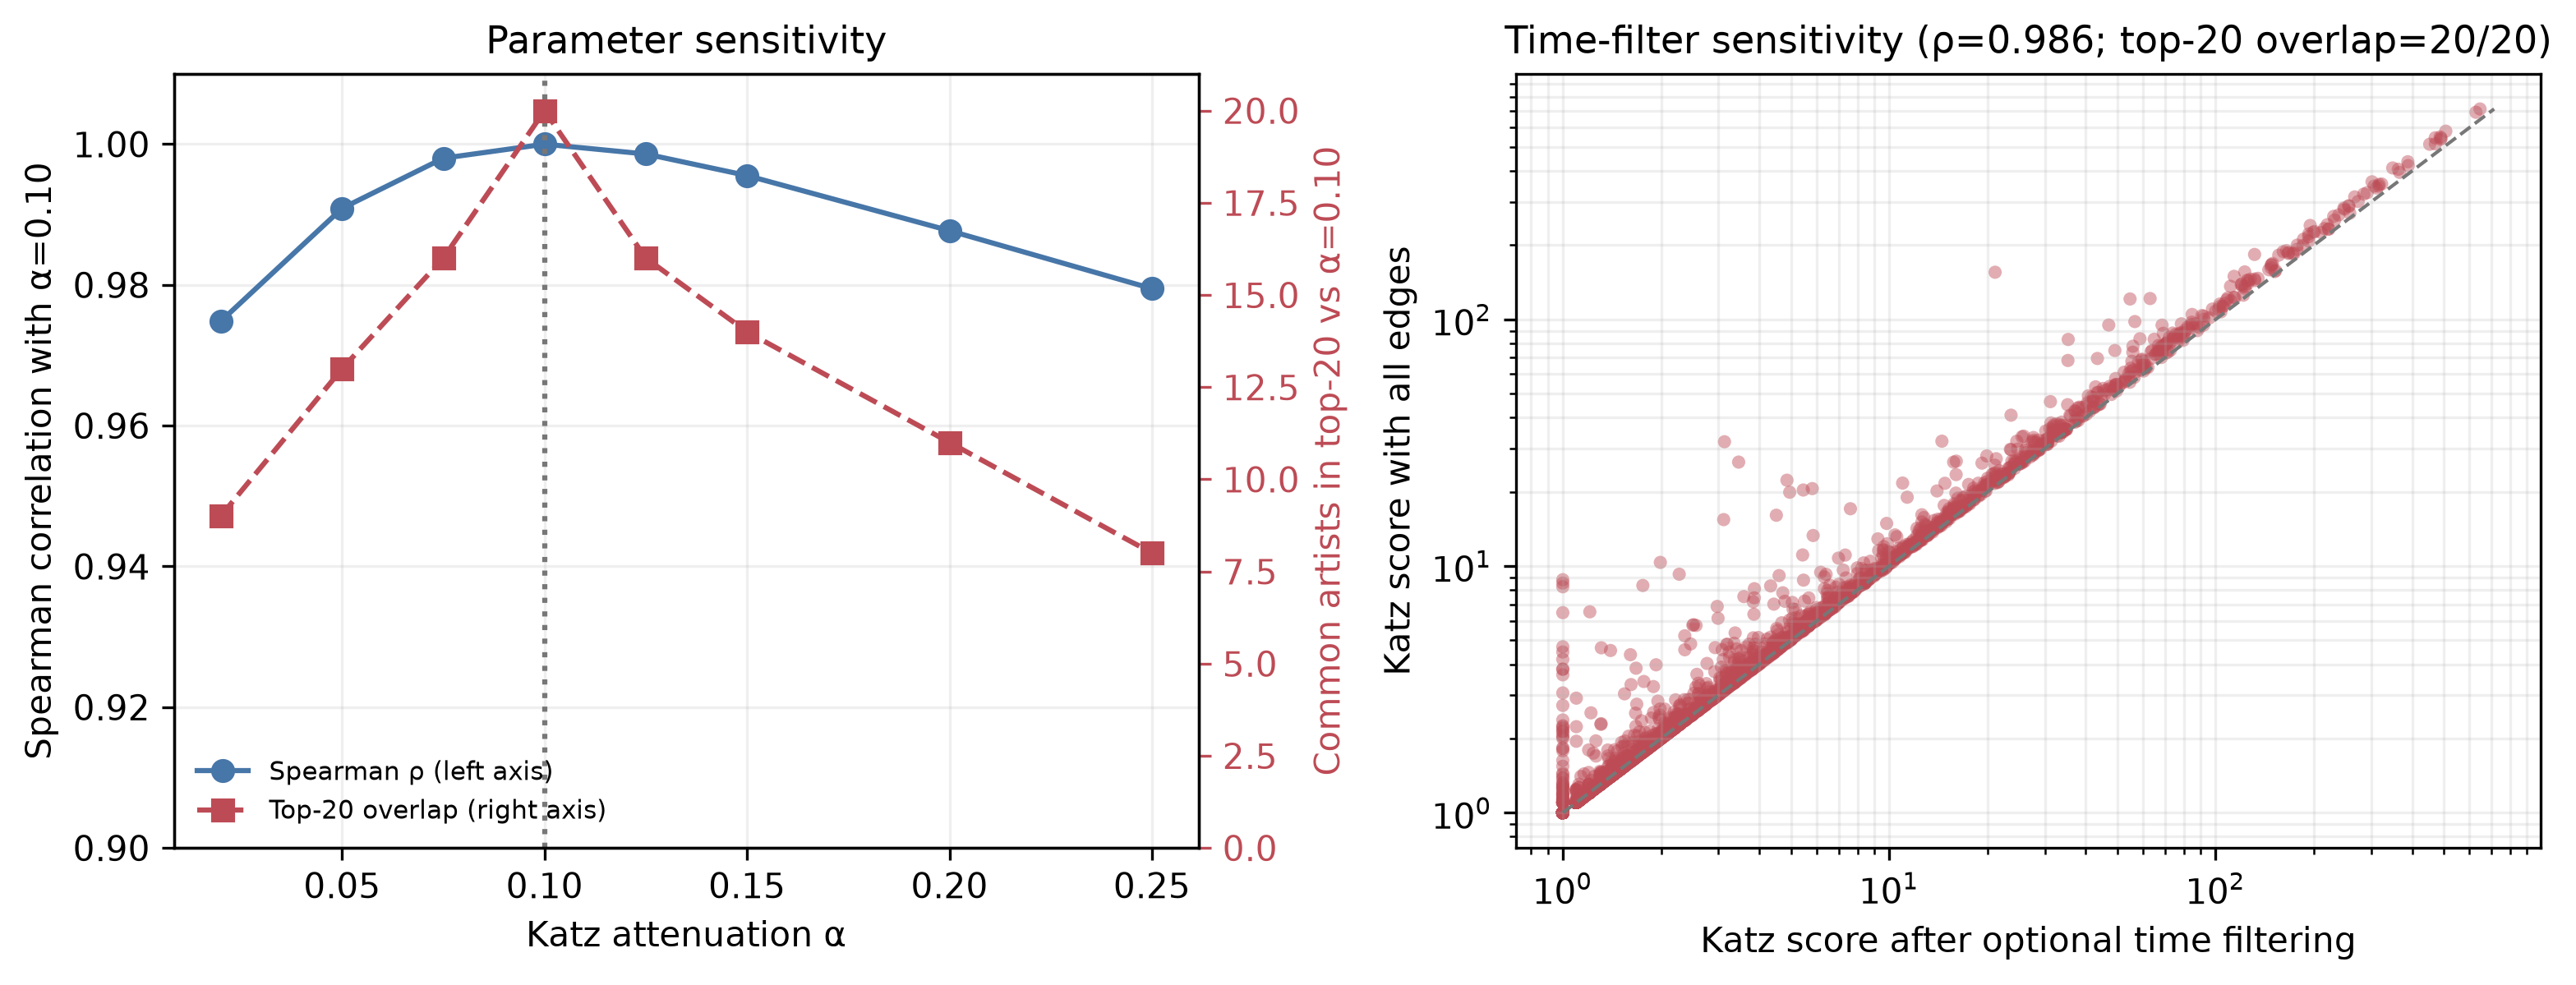
\includegraphics[width=0.95\textwidth]{fig2_sensitivity.png}
\caption{Robustness of the Katz ranking. \emph{Left:} sensitivity to the
attenuation factor: Spearman correlation between the baseline ranking
(\(\alpha=0.10\), dotted line) and rankings recomputed at other levels
(blue, left axis), and the number of artists common to the top-20 of both
rankings (red, right axis); both are maximised at the operating point.
\emph{Right:} per-artist Katz scores with all edges versus scores after
removing the 733 time-order-reversed edges; the dashed line marks equality.}
\label{fig:q1-sensitivity}
\end{figure}

Finally, the three measures corroborate one another in bulk (pairwise
Spearman $\rho$ between 0.95 and 0.97) while their top-20 sets overlap in
only 4--8 of 20 names---high bulk agreement with low top-rank overlap is
precisely the signature of a stable shared backbone topped by artists
specialised for different roles, which supports reporting the measures
separately instead of collapsing them into one index. Across all measures
we emphasise that edges are \emph{reported} relationships, not established
causal influence.




\section{Model II: Measures of Music Similarity}\label{sec:model-similarity}

This section addresses the second requirement of Problem~C: developing a quantitative measure of musical similarity from audio features, and testing whether artists within the same genre are more similar than artists from different genres. We use the existing \texttt{main\_genre} labels in \texttt{influence\_data}; we do not redefine genres such as Pop/Rock.

\subsection{Feature Representation}

For each artist $i$, we form a feature vector $\mathbf{x}_i \in \mathbb{R}^{p}$ from \texttt{data\_by\_artist}, using the Spotify audio attributes
\[
\begin{aligned}
\{\,&\text{danceability},\ \text{energy},\ \text{valence},\ \text{tempo},\ \text{loudness},\\
&\text{acousticness},\ \text{instrumentalness},\ \text{liveness},\ \text{speechiness},\ \text{duration\_ms},\ \text{popularity}\,\}.
\end{aligned}
\]
Genre labels are attached by joining on \texttt{artist\_id} with \texttt{influence\_data}. The within-/between-genre test keeps only artists that have a genre label (here $n=5599$ after dropping missing/Unknown labels).

Because these coordinates have incompatible scales (e.g., tempo versus danceability in $[0,1]$), we apply column-wise $z$-score standardization before any distance computation:
\[
\tilde{x}_{ik} = \frac{x_{ik}-\mu_k}{\sigma_k},\qquad k=1,\dots,p.
\]
All distances below are computed in this standardized space.

\subsection{Baseline Measure: Euclidean Distance}

As the primary similarity model, we measure stylistic discrepancy by Euclidean distance. For artists $i$ and $j$,
\[
d_{ij} = \bigl\|\tilde{\mathbf{x}}_i - \tilde{\mathbf{x}}_j\bigr\|_2 = \sqrt{\sum_{k=1}^{p}(\tilde{x}_{ik}-\tilde{x}_{jk})^2}.
\]
Smaller $d_{ij}$ means greater musical similarity. When a bounded score is useful for visualization, we may use $s_{ij}=1/(1+d_{ij})$; the formal within-/between comparison is performed on distances.

\paragraph{Why Euclidean distance.}
After standardization, Euclidean distance has a clear geometric reading (``closer points sound more alike''), is easy to reproduce in code, and maps directly onto the within-versus-between question. We emphasize that this is a \emph{distance}, not a correlation coefficient.

\subsection{Within-Genre versus Between-Genre Test}

Let $\mathcal{G}(i)$ denote the main genre of artist $i$. Define the average within-genre and between-genre distances
\[
\bar{d}_{\mathrm{within}}
  = \frac{1}{|W|}\sum_{(i,j)\in W} d_{ij},
\qquad
\bar{d}_{\mathrm{between}}
  = \frac{1}{|B|}\sum_{(i,j)\in B} d_{ij},
\]
where $W$ collects same-genre pairs and $B$ collects cross-genre pairs (pairs are randomly subsampled for computational tractability; seed fixed for reproducibility).

\textbf{Hypothesis.} If the feature geometry aligns with the provided genre taxonomy, we expect
\[
\bar{d}_{\mathrm{within}} < \bar{d}_{\mathrm{between}}.
\]
Empirically, under the standardized Euclidean baseline we obtain
\[
\bar{d}_{\mathrm{within}} \approx 3.73
\quad < \quad
\bar{d}_{\mathrm{between}} \approx 4.55.
\]
Thus the inequality holds globally. Large heterogeneous labels such as Pop/Rock may still show weaker within-genre cohesion than smaller, tighter genres.

To visualize genre neighbourhoods, we also compute each genre's centroid in the standardized feature space and plot the pairwise Euclidean distances between centroids (Figure~\ref{fig:heatmap-baseline}). The diagonal is zero by construction; brighter cells indicate nearer genres (e.g., Latin--R\&B, Country--Latin), while Comedy/Spoken is far from most musical genres.

\begin{figure}[t]
  \centering
  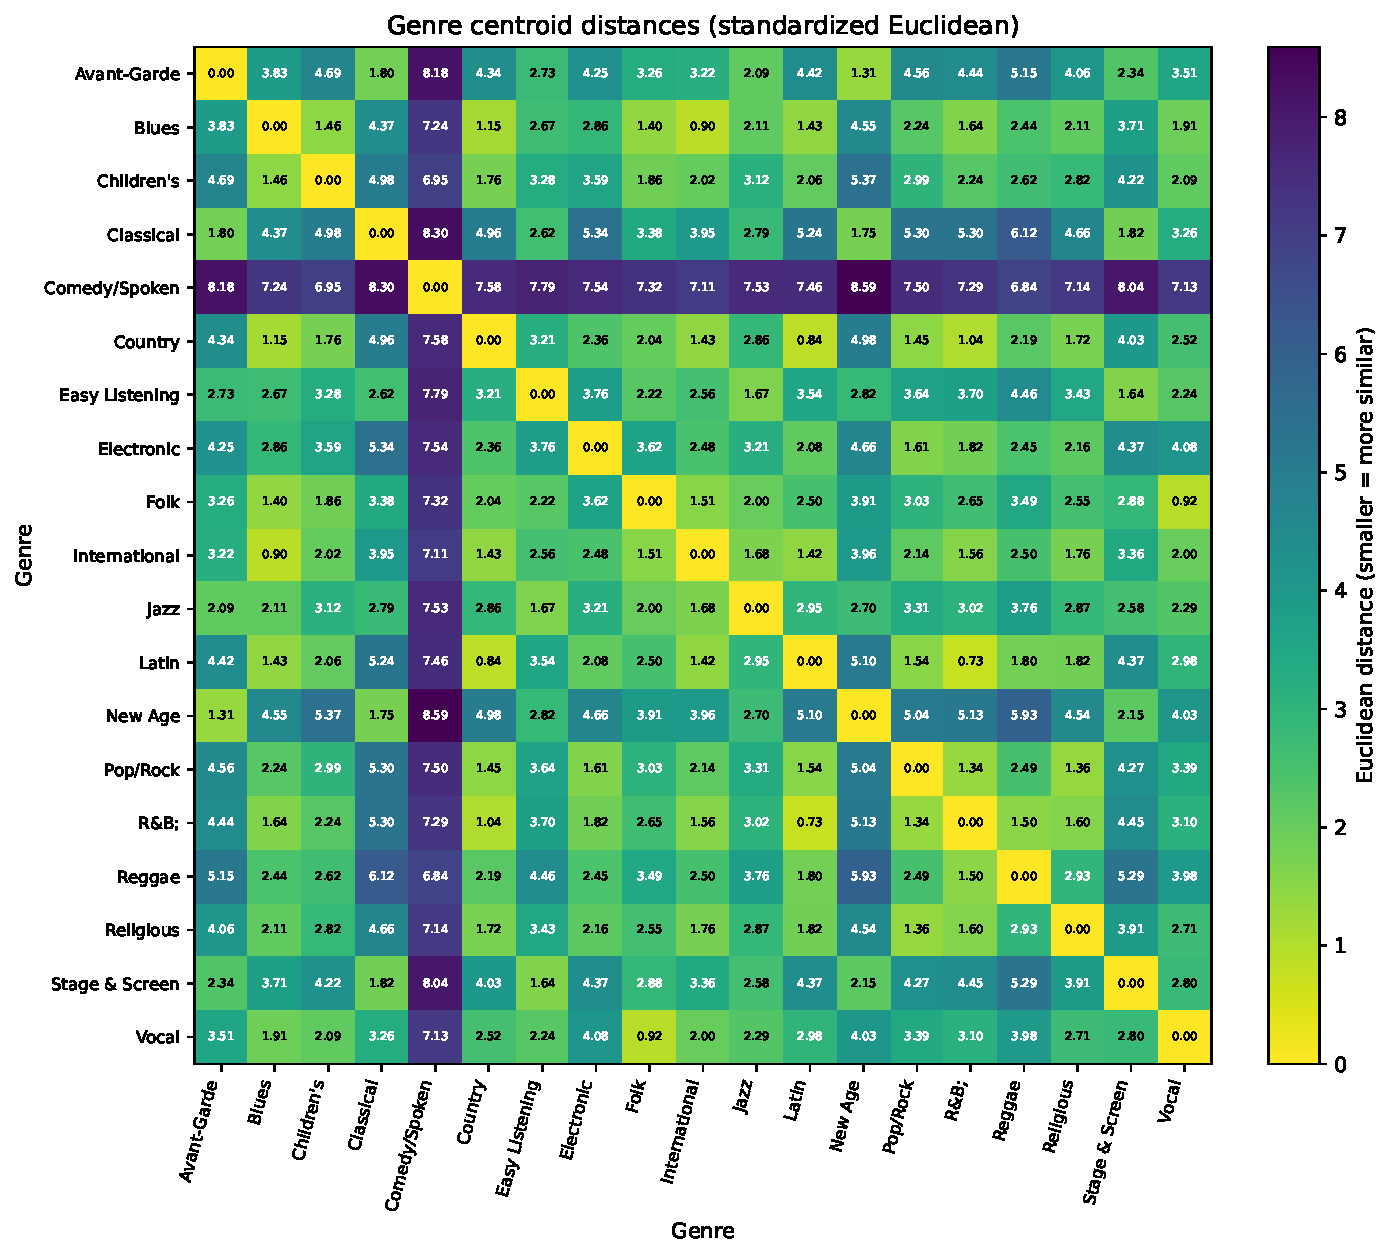
\includegraphics[width=0.62\textwidth]{heatmap_genre_distances_baseline.pdf}
  \caption{Pairwise Euclidean distances between genre centroids in $z$-scored feature space (brighter $=$ more similar).}
  \label{fig:heatmap-baseline}
\end{figure}

\subsection{Robustness Check: PCA then Euclidean Distance}

Audio features are correlated (e.g., energy and loudness), so Euclidean distance in the full standardized space can overweight redundant directions. As a second specification we: (i)~standardize; (ii)~apply PCA retaining enough components to explain at least $80\%$ of variance (here $r=6$, explaining about $82.5\%$); (iii)~recompute Euclidean distances in the score space; (iv)~repeat the within-/between comparison.

Under PCA$\to$Euclidean we again find
\[
\bar{d}_{\mathrm{within}} \approx 3.28
\quad < \quad
\bar{d}_{\mathrm{between}} \approx 4.10,
\]
so the qualitative conclusion is unchanged.

\subsection{Interim Conclusions for Model II}
\begin{itemize}
  \item Musical similarity is operationalized by standardized Euclidean distance on artist-level Spotify features, with PCA$+$Euclidean as a robustness check.
  \item Genres are taken from the dataset; we do not invent new genre definitions.
  \item Both specifications satisfy $\bar{d}_{\mathrm{within}}<\bar{d}_{\mathrm{between}}$.
  \item Similarity is not influence: a small $d_{ij}$ does not imply a declared influence edge (examined later when validating influencers against followers).
\end{itemize}


\section{Model III: Genre Comparison, Distinction and Change}\label{sec:model-genre}

This section addresses the genre-level questions of Problem~C: comparing
similarities (and, with Model~I, influences) within and between genres;
asking what distinguishes a genre; asking how genres change over time; and
asking whether some genres are related to others. Throughout we keep a
single genre representation so that the subsections stay coherent.

\subsection{Genre Representation: Katz-Weighted Feature Centroids}\label{subsec:q3-centroids}

Let \(\tilde{\mathbf{x}}_i\in\mathbb{R}^{p}\) be the globally \(z\)-scored
Spotify feature vector of artist \(i\) (the same \(p=11\) coordinates and
standardization as Model~II), and let \(K_i\) be the outgoing Katz score
from Model~I. For each official main genre \(g\) we define the
\emph{influence-weighted} genre vector
\begin{equation}\label{eq:cg}
\mathbf{c}_g
=\frac{\sum_{i:\,\mathcal{G}(i)=g} K_i\,\tilde{\mathbf{x}}_i}
      {\sum_{i:\,\mathcal{G}(i)=g} K_i}.
\end{equation}
Artists who transmit influence more broadly therefore pull the genre
profile more strongly. An equal-weight centroid is retained only as a
robustness check (off-diagonal correlation of the two distance matrices
\(\approx 0.73\)). After joining Model~II features to Model~I scores we
obtain \(n=5599\) artists across 19 genres.

Between-genre discrepancy is the Euclidean distance
\(d_{gh}=\|\mathbf{c}_g-\mathbf{c}_h\|_2\), with bounded similarity
\(s_{gh}=1/(1+d_{gh})\). Within-genre cohesion is the (Katz-weighted) mean
distance of artists in \(g\) to \(\mathbf{c}_g\). Empirically the mean
within-genre cohesion is \(2.92\), below the mean between-genre centroid
distance \(3.79\): genres remain separated at the aggregate level even
after influence weighting. The closest pairs are Blues--R\&B
(\(d\approx 0.76\)), Blues--Country (\(0.78\)) and Latin--R\&B (\(0.86\));
the farthest involve Avant-Garde against Comedy/Spoken, Children's and
Country (\(d>8\)).

\begin{figure}[t]
\centering
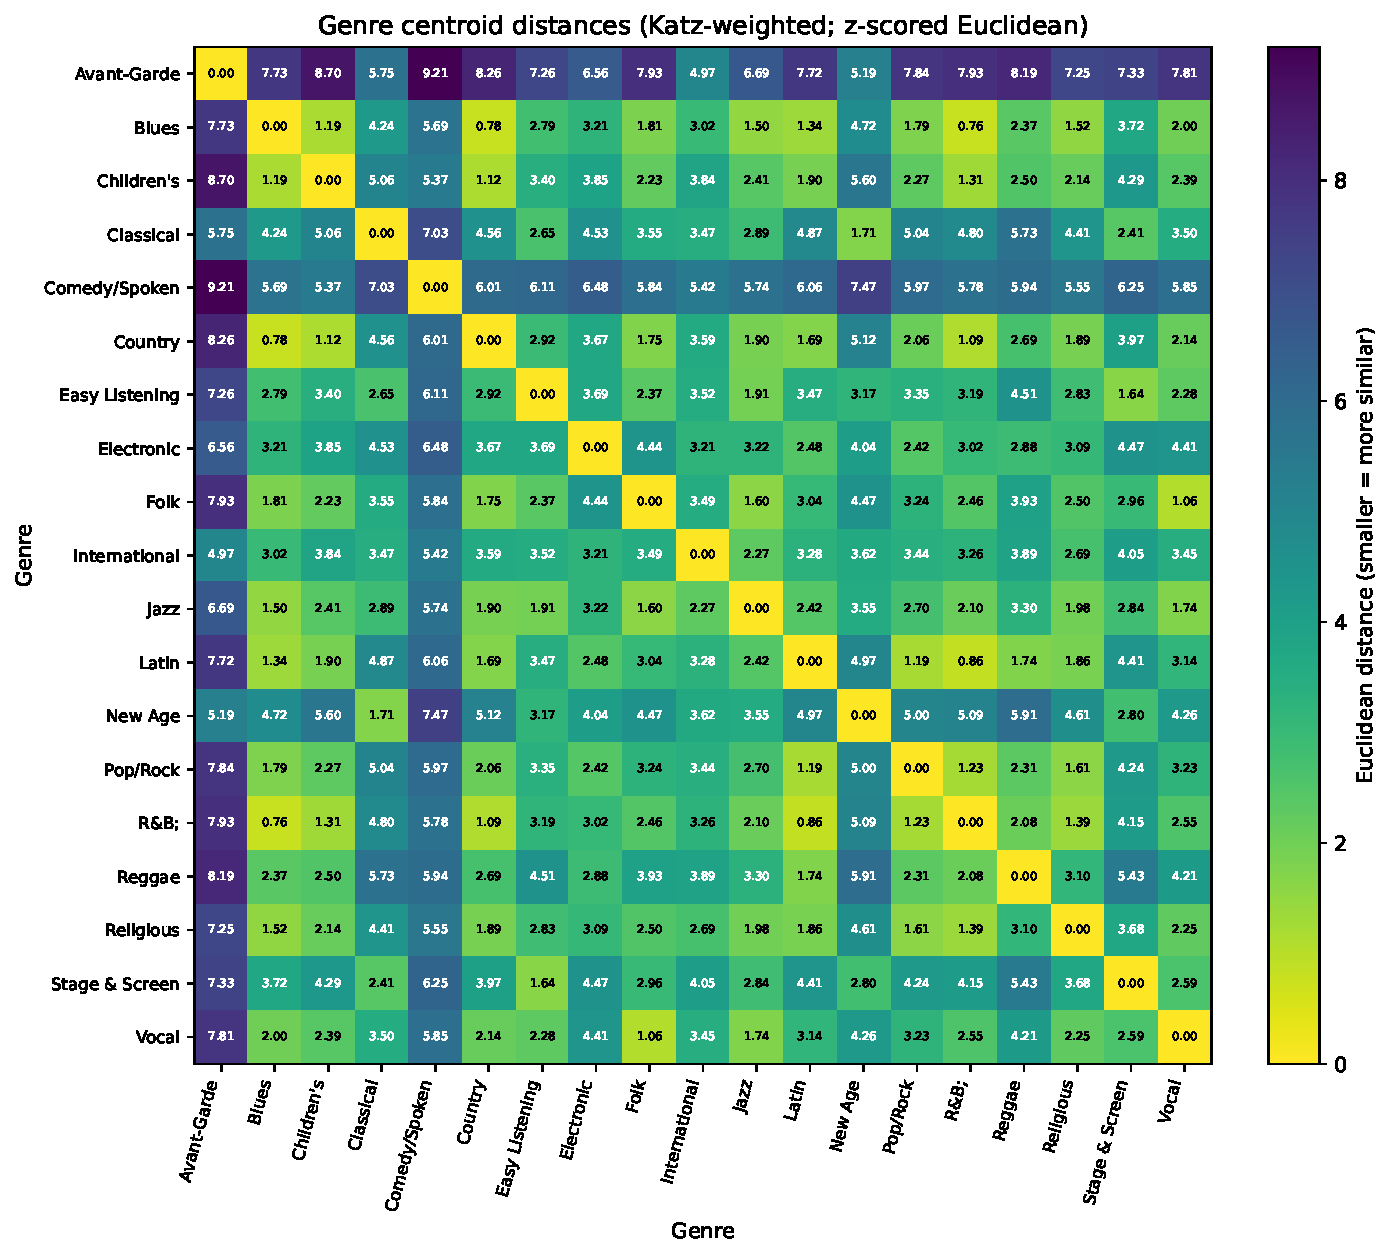
\includegraphics[width=0.65\textwidth]{heatmap_genre_distances_katz.pdf}
\caption{Pairwise Euclidean distances between Katz-weighted genre
centroids \(\mathbf{c}_g\) (smaller $=$ more similar).}
\label{fig:q3-genre-dist}
\end{figure}

\subsection{What Distinguishes a Genre?}\label{subsec:q3-distinguish}

We do \emph{not} assign each genre a unique exclusive feature: with
\(p=11\) features and 19 genres that would be neither feasible nor
meaningful. Instead we read the \emph{same} vectors \(\mathbf{c}_g\). In
\(z\)-space each coordinate of \(\mathbf{c}_g\) is already a signed
deviation from the all-artist mean, so a genre is distinguished by its
\emph{profile}---which coordinates are high or low together.
The most discriminating coordinates globally are
\texttt{duration\_ms}, \texttt{speechiness}, \texttt{instrumentalness}
and \texttt{valence}. Extreme profiles include Avant-Garde (very long
duration), Comedy/Spoken (very high speechiness) and Classical / New~Age
(high instrumentalness and acousticness, low loudness/energy). By
contrast Pop/Rock, Latin and R\&B lie closest to the global mean
(\(\|\mathbf{c}_g\|_2\) small), consistent with coarse, heterogeneous
labels. Even near neighbours remain separable by a few coordinates: e.g.\
Blues versus R\&B differ mainly in loudness, energy and acousticness.

\subsection{How Genre Similarity Changes over Time}\label{subsec:q3-sim-time}

To study change we keep the definition~\eqref{eq:cg} but index it by the
artist's active-start decade \(t\) (Assumption~A2): \(\mathbf{c}_g(t)\) is
formed from artists of genre \(g\) who \emph{began} in decade \(t\), still
weighted by the Model~I Katz score, in the same global \(z\)-space. A
genre enters decade \(t\) only if at least five such artists are present.
We treat 1950--2000 as the main window; the 1930s and especially the
2010s are sparse (only four genres meet the threshold in the 2010s).

\begin{figure}[t]
\centering
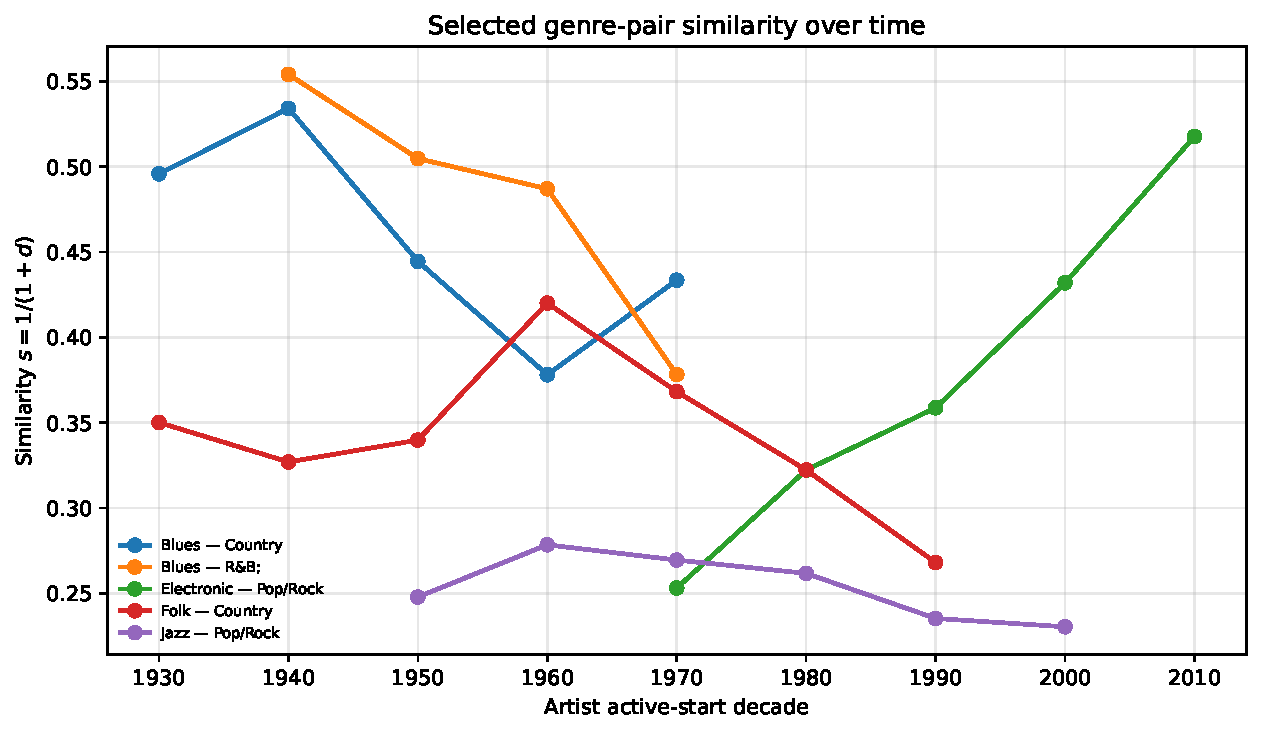
\includegraphics[width=0.65\textwidth]{genre_pair_similarity_over_time.pdf}
\caption{Similarity \(s=1/(1+d)\) for selected genre pairs over decades.
Electronic--Pop/Rock becomes more similar; Blues--R\&B and Folk--Country
trend slightly apart where both are observed.}
\label{fig:q3-pair-time}
\end{figure}

Mean between-genre distance rises from about \(3.16\) (1950s) to about
\(4.55\) (2000s): later cohorts are, on average, more sonically separated.
Pairwise trajectories are heterogeneous---Electronic and Pop/Rock move
closer (\(\Delta s\approx +0.18\) from the 1970s to the 2000s), while
Blues--R\&B similarity falls over the decades in which both are observed.
Self-drift \(\|\mathbf{c}_g(t)-\mathbf{c}_g\|\) is largest for
Comedy/Spoken, International and Classical, indicating that their
decade-specific weighted profiles move farthest from the static
\(\mathbf{c}_g\).

\subsection{How Genre Influence Changes over Time}\label{subsec:q3-inf-time}

% ---------------------------------------------------------------------------
% PLACEHOLDER — teammate (Model I / network side); filled via
% model3_s74_s75_supplement.tex when that file is \input from main.
% ---------------------------------------------------------------------------
\textbf{[Teammate TODO --- genre influence over time.]}
Using the directed network of Model~I, quantify how \emph{influence}
among genres evolves by active-start decade (or edge-endpoint decade):
e.g.\ cross-genre edge counts / share, genre-level outgoing Katz mass, and
export from one genre into another. Place the resulting time series next
to \cref{fig:q3-pair-time} and discuss where sonic similarity and
reported influence move together or diverge.
% End placeholder.

\subsection{Are Some Genres Related to Others?}\label{subsec:q3-related}

% ---------------------------------------------------------------------------
% PLACEHOLDER — synthesize similarity (done) with influence (teammate)
% Can reuse fig:q3-genre-dist and closest/farthest pairs; add a joint
% scatter or two-panel figure: similarity vs cross-genre influence.
% ---------------------------------------------------------------------------
\textbf{[TODO --- relatedness synthesis.]}
The distance matrix in \cref{fig:q3-genre-dist} already supplies a sonic
relatedness graph (Blues--R\&B--Country--Latin as a close cluster;
Avant-Garde as an outlier). Complete this subsection by combining that
picture with Model~I cross-genre influence: genres may be (i)~sonically
close and strongly cross-linked, (ii)~sonically close but weakly linked,
or (iii)~sonically far yet heavily cross-influencing. A short taxonomy of
a few genre pairs under these three regimes answers whether ``related''
should mean sound-alike, citation-linked, or both.
% End placeholder.

% ============================================================================
% Paste-ready supplement for Model III (replaces the two TODO placeholders in
% model3.tex). Style, labels and notation follow the joint report:
%   \mathcal{G}(i) genre map, \cref cross-references, booktabs tables.
% Figure file required: genre_influence_over_time.pdf (panel (a)(b), compact,
%   sits next to \cref{fig:q3-pair-time}).
% ============================================================================

\subsection{How Genre Influence Changes over Time}\label{subsec:q3-inf-time}

While \cref{subsec:q3-sim-time} tracks how \emph{sonic similarity} between
genres evolves, this subsection quantifies how \emph{reported influence}
between genres evolves. We do not build a second network: the genre-level
flows are obtained by \emph{aggregating} the artist-level network of
Model~I over the genre partition, exactly as the Katz-weighted centroids
of \cref{subsec:q3-centroids} aggregate the feature vectors. For each pair
of main genres $(g,h)$ we count
\begin{equation}\label{eq:F-gh}
F_{gh} \;=\; \sum_{(i,j)\in E}\,
\mathbb{1}\!\left[\mathcal{G}(i)=g\right]\,
\mathbb{1}\!\left[\mathcal{G}(j)=h\right],
\end{equation}
the number of reported edges from genre-$g$ influencers to genre-$h$
followers. The construction is a deterministic group-by on the cleaned
edge table of section~4.2, so it introduces no new edge definition and no
new parameters. Its correctness is guaranteed by the conservation identity
$\sum_{g,h}F_{gh}=|E|=42{,}770$ (including the $733$ time-reversed edges
retained under Assumption~A3; excluding them gives $42{,}037$), which we
verify explicitly, and by an exact match of the Jazz$\to$Pop/Rock block
with the subnetwork count of section~5.6 ($409$ edges; $406$ when the
three reversed edges among them are excluded). All counts in this
subsection follow the same convention. Row- and column-normalized variants,
$P_{gh}=F_{gh}\big/\sum_{h'}F_{gh'}$ and
$Q_{gh}=F_{gh}\big/\sum_{g'}F_{g'h}$, express the \emph{export profile} of
$g$ and the \emph{source profile} of $h$; the normalization removes the
strong size effect of the genre labels (Pop/Rock alone carries $56\%$ of
all edges, section~4.4) and leaves pure flow structure.

The time dimension follows the cohort convention of section~5.5:
$F_{gh}(t)$ restricts \eqref{eq:F-gh} to edges whose \emph{follower}
started in decade $t$ (1930--2010; decades with fewer than $50$ edges are
omitted). As in \cref{subsec:q3-sim-time} we treat 1950--2000 as the main
window; the 1930s and 2010s cohorts are thin (193 and 811 edges) and are
read only with that caveat. We emphasize that this conditioning variable
differs from
\cref{subsec:q3-sim-time}, which indexes artists by their \emph{own}
active-start decade: there $\mathbf{c}_g(t)$ describes the sound of genre
$g$'s generation $t$, here $F(t)$ describes what generation $t$
\emph{absorbed}. The two curves of \cref{fig:q3-pair-time} and
\cref{fig:q3-inf-time} are therefore complementary readings of the same
timeline.

\paragraph{Cross-genre influence rises, peaks, and settles into a
plateau.} Let
$c(t)=1-\sum_g F_{gg}(t)\big/\sum_{g,h}F_{gh}(t)$ denote the cross-genre
share of edges received by generation $t$ (panel~(a) of
\cref{fig:q3-inf-time}). The share climbs from $0.23$ (1940s cohort) to a
peak of $0.37$ for the 1960s cohort---the era in which Blues, R\&B,
Country and Pop/Rock most heavily cross-fed, consistent with the birth of
rock---and then falls to a stable plateau of $0.18$ across the
1980s--2000s cohorts (the thin 2010 cohort ticks up to $0.23$). In terms
of raw reported edges, later generations drew an increasingly
\emph{within-genre} diet.

\paragraph{Quantity and quality of cross-genre influence diverge.} The raw
share treats all followers equally. Re-weighting each edge by the
follower's outgoing Katz score $K_j$ from Model~I---influencing a future
hub counts for more---produces the Katz-weighted share $c_K(t)$ (blue
dashed curve of panel~(a)). Its maximum shifts a full decade earlier:
$c_K(t)$ peaks at $0.53$ for the 1950s cohort and collapses below $0.19$
for every cohort from the 1970s through the 2000s (the thin 2010 cohort
ticks back up to $0.23$). The divergence between the two curves is itself
informative: among early post-war artists, those who absorbed cross-genre
influence went on to become disproportionately influential themselves,
whereas among artists active from the 1970s onward, cross-genre followers
are on average \emph{less} connected to future influence than same-genre
followers. The era of maximum cross-genre \emph{traffic} (1960s) precedes
the era of maximum cross-genre \emph{leverage} (1950s).

\paragraph{Selected flows.} Panel~(b) plots the export share $P_{gh}(t)$
for five informative pairs (genre-decade rows with at least $20$ edges are
shown). Three patterns stand out.
(i)~\emph{Jazz steadily redirects its influence outward}: its export share
toward Pop/Rock rises overall from $0.05$ (1950s cohort) to $0.35$ (2000s
cohort)---holding at $0.20$--$0.23$ across the 1960s--1980s cohorts with a
dip to $0.20$ in the 1990s---while the Jazz$\to$Jazz block
shrinks---jazz increasingly feeds mainstream genres rather than its own
tradition. (The 2010 cohort is omitted from panel~(b): it contains only
three Jazz edges.)
(ii)~\emph{Blues--R\&B decouples}: Blues' export share toward R\&B is
$0.23$ for the 1930s cohort---five edges, out of an R\&B inflow of just
seven, so Blues supplied $71\%$ of everything the first R\&B cohort
received---but the share falls below $0.16$ already in the 1940s and to
$0$--$6\%$ across the 1980s--1990s cohorts (on $41$--$78$ edges); what
remains afterwards is small-sample noise ($0.19$ in the 2000 cohort
represents four edges). The pattern reflects the diversification of R\&B's
sources as the genre broadened.
(iii)~\emph{Electronic enters late and feeds Pop/Rock strongly}: the flow
only appears in the 1970s (the genre itself barely exists before then) and
immediately dominates Electronic's export profile ($0.70$ for the 1970s
cohort, $0.50$ for the 2000s cohort).

\paragraph{Where similarity and influence move together or diverge.}
Reading \cref{fig:q3-inf-time} against \cref{fig:q3-pair-time} shows that
the two lenses agree only partially.
\emph{Together}: Electronic--Pop/Rock both converges in sound
($\Delta s\approx+0.18$ in \cref{subsec:q3-sim-time}) and dominates
Electronic's export profile---sonic convergence here tracks reported
influence.
\emph{Diverging, influence ahead of sound}: Jazz's export share toward
Pop/Rock rises overall ($0.05\to0.35$, with a 1990s dip) while the
Jazz--Pop/Rock
similarity stays flat or drifts slightly down ($0.25\to0.23$); reported
influence deepened even as the two profiles drifted apart.
\emph{Diverging, influence behind sound}: Blues--R\&B is the sonically
closest pair of the whole system ($d=0.76$ in \cref{subsec:q3-centroids}),
yet Blues' export share toward R\&B fell from $0.23$ to $0$--$6\%$ across
the 1980s--1990s cohorts; closeness of sound did not preserve closeness of
reported influence.
Sonic similarity is thus neither necessary nor sufficient for reported
influence---the two measures answer different questions, which is why we
keep both.

\paragraph{Where the influence mass sits.} A complementary,
follower-independent view aggregates the artists themselves:
$K_g(t)=\big(\textstyle\sum_{i:\,\mathcal{G}(i)=g,\,
\mathrm{start}(i)=t}K_i\big)\big/
\big(\textstyle\sum_{i:\,\mathrm{start}(i)=t}K_i\big)$, the share of
generation $t$'s outgoing-Katz mass held by genre $g$. Pop/Rock rises from
negligible mass in the 1930s to $0.73$--$0.75$ for the 1960s--1980s
cohorts and remains dominant; Jazz collapses from $0.24$ (1930s) to
$0.01$ (1980s onward); Electronic grows from zero to ${\approx}\,0.08$.
The genre system concentrated its influence-carrying capacity into
Pop/Rock precisely during the decades in which its cross-genre
\emph{intake} fell---consolidation of output accompanied consolidation of
input.

\begin{figure}[htbp]
\centering
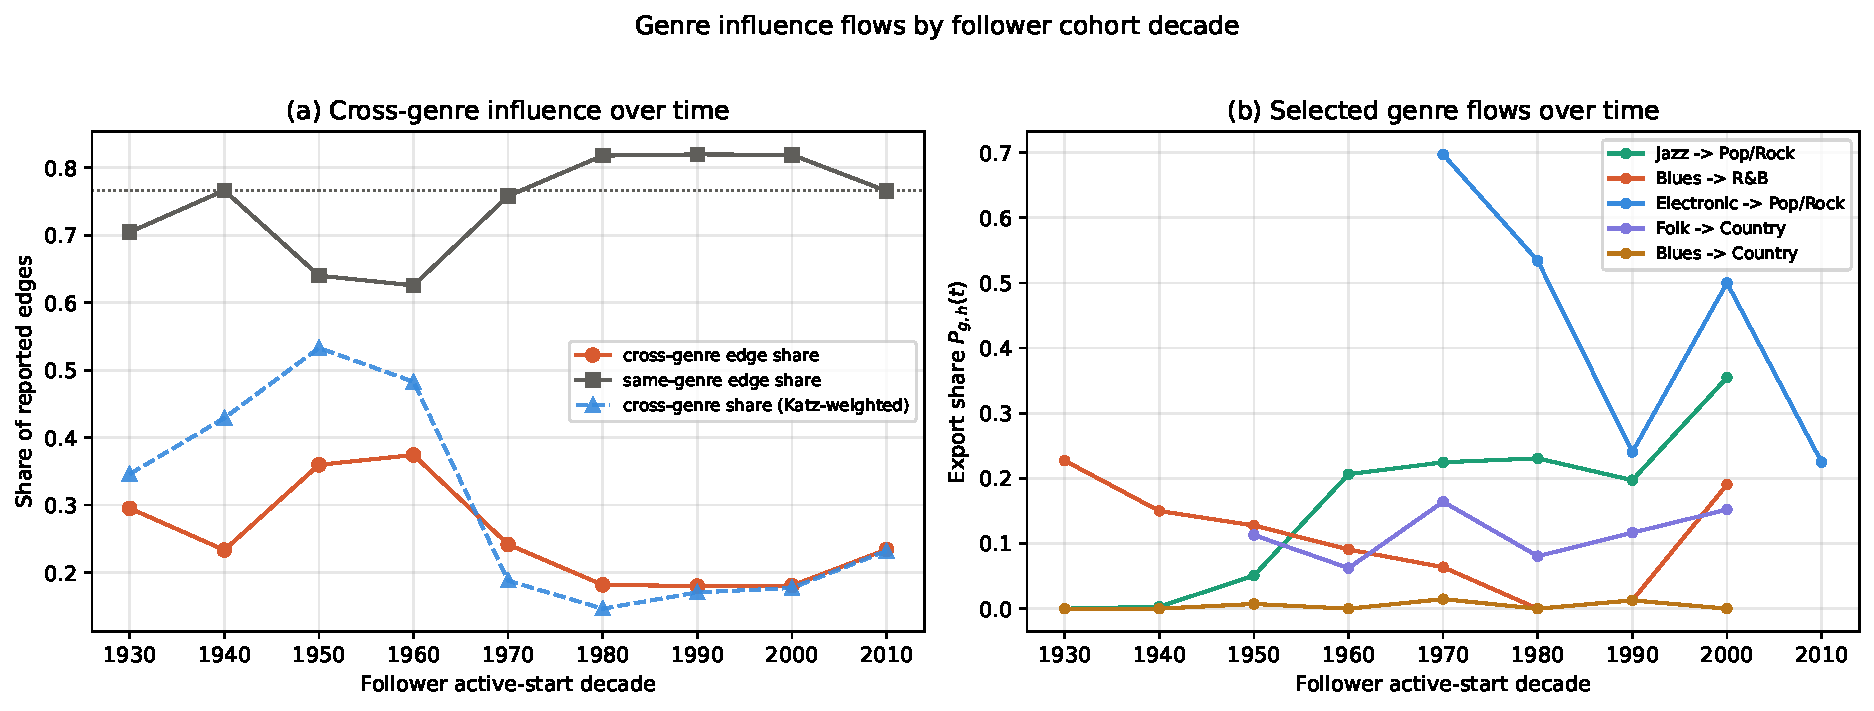
\includegraphics[width=0.98\textwidth]{genre_influence_over_time.pdf}
\caption{Genre influence flows by follower cohort decade.
(a)~Cross-genre share of edges $c(t)$ (red) against the same-genre share
(grey; dotted line marks the all-network value $0.766$), and the
Katz-weighted cross-genre share $c_K(t)$ (blue dashed).
(b)~Export share $P_{gh}(t)$ for five selected flows; points are shown
only for genre-decade rows with at least $20$ edges.}
\label{fig:q3-inf-time}
\end{figure}

\paragraph{Robustness and disclosure.} The matrices retain edges whose
labels are \texttt{Unknown} so that the conservation identity holds
exactly; the discussion above concerns the 19 named genres. Retaining the
733 time-reversed edges follows Assumption~A3, and their impact is
quantified in section~5.7; removing them changes the decade cross-genre
shares by at most $0.023$ (1930s cohort, the smallest sample) and by no
more than $0.01$ for every decade from the 1940s onward, so no conclusion
moves. The Katz-weighted curve $c_K(t)$ uses the same attenuation
$\alpha=0.10$ as Model~I; the artist-level attenuation scan of
section~5.7 (rank correlation ${\ge}\,0.975$ over
$\alpha\in[0.05,0.20]$) supports that reweighting with a different
$\alpha$ would not alter the shape of panel~(a).

Two significance checks back the shape of panel~(a). First, a
\emph{permutation test} addresses the concern that decade-to-decade moves
in $c_K(t)$ merely track the changing genre composition of each cohort:
within each decade we shuffle the influencer genre labels (1{,}000
draws), which keeps the cohort's edge count, genre mix and follower Katz
weights fixed while destroying any real genre homophily. Observed
$c_K(t)$ lies far \emph{below} the composition-adjusted null in every
cohort---genres are homophilous in whom they cite---but the excess
homophily is precisely what carries the story: it is weakest for the
1950s--1960s cohorts ($z\approx-10$ to $-21$) and strongest from the
1980s onward ($z\le-45$; all one-sided $p<0.001$). The mid-century peak
in cross-genre influence is therefore not an artifact of which genres
happened to be large at the time.

\subsection{Are Some Genres Related to Others?}\label{subsec:q3-related}

\cref{subsec:q3-centroids} supplies a \emph{sonic} relatedness picture
($d_{gh}$, \cref{fig:q3-genre-dist}); \cref{subsec:q3-inf-time} supplies a
\emph{reported-influence} picture ($F_{gh}$ and $P_{gh}$). Joining them
yields a simple typology of genre relatedness. A \emph{Mantel test}
correlating the off-diagonal entries of the sonic-distance matrix with
those of the symmetric cross-flow matrix ($F_{gh}+F_{hg}$,
log-scaled) gives $r=-0.41$ with permutation $p=0.0008$
($5{,}000$ row/column permutations): reported influence decays with sonic
distance, and every one of the strongest cross-links
(${\ge}\,200$ edges) lies at moderate distance
($1.2\le d\le 3.2$). Three regimes emerge
(\cref{tab:q3-related-types}).

\emph{(i)~Sonically close and strongly cross-linked.} Pop/Rock--R\&B
($d=1.23$, $1{,}909$ cross edges) is the dominant corridor of the whole
network, followed by Country--Pop/Rock ($2.06$; $1{,}160$),
Electronic--Pop/Rock ($2.42$; $801$), Blues--Pop/Rock ($1.79$; $736$) and
Latin--Pop/Rock ($1.19$; $235$). These are pairs whose sound is similar
\emph{and} whose artists cite each other heavily: relatedness in both
senses at once.

\emph{(ii)~Sonically close but weakly linked.} Blues--Country
($d=0.78$ but only $16$ cross edges), Latin--R\&B ($0.86$; $39$),
Country--R\&B ($1.09$; $46$) and Folk--Vocal ($1.06$; $19$) are sonic
siblings that rarely cite each other directly. Their resemblance is
plausibly a shared ancestry---both grew from common roots---rather than
an active exchange documented in the data.

\emph{(iii)~Sonically far yet influential---only in relative terms.} No
distant pair clears the $200$-edge bar: at the level of raw counts,
sonically remote genres barely interact. The share view
($Q_{gh}$) reveals a weaker form of the regime confined to niche genres
with thin inflows: Pop/Rock supplies $31\%$ of the (small) influence
received by Classical ($d=5.04$), and Pop/Rock dominates the inflows of
Avant-Garde ($30\%$, $d=7.84$) and New~Age ($19\%$, $d=5.00$). These are
cases where one mainstream donor towers over a shallow pool, not genuine
long-range channels.

The typology also exposes a strong \emph{hub asymmetry}: Pop/Rock
accounts for $45\%$ of everything Electronic receives, while the reverse
flow is $1.1\%$ of what Pop/Rock receives ($504$ vs.\ $297$ edges). In
the reported network, influence is not exchanged between equals---it is
donated by the hub, and the hub barely records what it takes in.

\begin{table}[htbp]
\centering
\small
\caption{Relatedness typology from sonic distance $d_{gh}$
(\cref{fig:q3-genre-dist}) and reported cross-genre edges
($F_{gh}+F_{hg}$). Type~(iii) examples are shown with the donor's share
$Q_{gh}$ of the receiver's inflow, since their absolute counts are small.}
\label{tab:q3-related-types}
\begin{tabular}{llrl}
\toprule
Type & Pair & $d_{gh}$ & Evidence \\
\midrule
(i) close \& strongly linked
  & Pop/Rock--R\&B        & $1.23$ & $1{,}909$ cross edges \\
  & Country--Pop/Rock     & $2.06$ & $1{,}160$ cross edges \\
  & Electronic--Pop/Rock  & $2.42$ & $801$ cross edges \\
  & Blues--Pop/Rock       & $1.79$ & $736$ cross edges \\
\addlinespace
(ii) close \& weakly linked
  & Blues--Country        & $0.78$ & $16$ cross edges \\
  & Latin--R\&B           & $0.86$ & $39$ cross edges \\
  & Country--R\&B         & $1.09$ & $46$ cross edges \\
\addlinespace
(iii) far \& influential (relative)
  & Pop/Rock $\to$ Classical    & $5.04$ & $31\%$ of inflow ($Q$) \\
  & Pop/Rock $\to$ Avant-Garde  & $7.84$ & $30\%$ of inflow ($Q$) \\
  & Pop/Rock $\to$ New Age      & $5.00$ & $19\%$ of inflow ($Q$) \\
\bottomrule
\end{tabular}
\end{table}

% ============================================================================
% Paste-ready Model V section for the MAT3300 report (Question 4:
% "Does similarity data support that the identified influencers actually
% influence the respective artists? Are some characteristics more
% contagious than others?")
%
% Requirements in the main document:
%   * figures/feature_contagion_excess.pdf   (fig11)
%   * figures/dose_response_excess.pdf       (fig12)
%   * booktabs, amsmath, graphicx, cleveref (already in the preamble)
% Labels follow the team convention: subsec:q4-*, eq:q4-*, fig:q4-*, tab:q4-*.
% ============================================================================

\section{Model IV: Does Influence Leave an Acoustic Trace?}\label{sec:model-q4}

The last question of Problem~C asks whether the similarity data actually
\emph{support} the influence relationships reported in
\texttt{influence\_data.csv}: do the ``influencers'' genuinely shape the
music of their followers, and are some musical characteristics more
\emph{contagious} than others? Model~II measures how similar two artists
sound; Model~I records \emph{who claimed to influence whom}. Neither
alone answers the question, because a high similarity along a reported
edge may simply reflect \emph{homophily}---followers choose their
influencers from artists they already sound like. This section therefore
combines the two models in a matched-control design: the reported edges
of Model~I are the treatment group, and statistically comparable
\emph{unrelated} artist pairs form the control group, so that any
excess resemblance along the edges can be attributed to the reported
influence rather than to selection.

\subsection{Matched-Control Excess Similarity}\label{subsec:q4-design}

Let $s(i,j)=1/(1+\lVert\tilde{\mathbf{x}}_i-\tilde{\mathbf{x}}_j\rVert_2)$
be the bounded similarity of Model~II in the global $z$-space
(\cref{subsec:q3-centroids}). For every reported edge $(i,j)$ of
Model~I we draw $K=10$ \emph{control} artists $j'$ matched to $j$ on the
two variables that drive homophily---main genre $\mathcal{G}(j')=
\mathcal{G}(j)$ and active-start decade $t(j')=t(j)$---with the
constraint that no edge $(i,j')$ exists in the influence data. The
\emph{excess similarity} of the edge is
\begin{equation}\label{eq:q4-excess}
s^{*}(i,j)=s(i,j)-\frac{1}{K}\sum_{k=1}^{K}s(i,j'_k),
\end{equation}
the resemblance along the edge beyond what the genre-and-decade baseline
predicts. A positive and significant $s^{*}$ means the follower's sound
is closer to the influencer than to comparable artists they did
\emph{not} choose---evidence \emph{consistent with} influence (the data
provide a single post-hoc snapshot per artist, so the design supports
consistency claims, not before/after causal proof; we use this wording
throughout).

All $42{,}770$ edges enter the test except $18$ edges whose endpoints
lack audio features and $55$ edges whose follower-genre/decade cell
contains no admissible control ($42{,}697$ edges analysed; the dropped
$0.17\%$ are disclosed rather than imputed). Features, standardization
and similarity are inherited from Model~II without modification, and the
edge table and decade convention are those of Model~I
(Assumption~A2); no new parameter enters except the control count $K$,
whose variation is discussed in the robustness paragraph.

\subsection{Do Influencers Actually Shape Their Followers?}\label{subsec:q4-overall}

The edges are systematically more similar than their controls: mean edge
similarity $0.286$ versus $0.250$ along matched controls, giving
$\bar{s}^{*}=0.0354$ with a bootstrap $95\%$ confidence interval
$[0.0347,\,0.0360]$ and a one-sided Wilcoxon $p<10^{-15}$;
$70.1\%$ of individual edges have $s^{*}>0$. The effect is modest in
absolute size---homophily explains most of the raw resemblance, as the
control construction makes visible---but it is extremely consistent:
reported influence carries a genuine acoustic signature that survives
matching on genre and era. We conclude that the similarity data
\emph{do} support the reported influence network.

\subsection{Which Characteristics Are Contagious?}\label{subsec:q4-features}

Repeating the matched-control comparison coordinate by coordinate
yields a per-feature excess
$a_f=\mathbb{E}[\,|\tilde{x}_j^{f}-\tilde{x}_{i}^{f}|\,]\text{ control minus edge}$,
reported in \cref{tab:q4-features} and \cref{fig:q4-features}.
The answer to ``are all characteristics equally contagious'' is a clear
\emph{no}: the gradient spans a factor of six. Style-defining
characteristics dominate---acousticness, valence, energy and
danceability all show excesses around $0.15$ in median
$z$-units---whereas technical or structural characteristics
(instrumentalness, speechiness, duration) show excesses an order of
magnitude smaller. Loudness and tempo occupy the middle ground. In
other words, followers absorb \emph{how the music feels} (texture,
mood, groove) far more reliably than \emph{how it is organised}.

The magnitude-versus-median contrast also flags distributional caveats:
instrumentalness has mean excess $0.121$ but median excess $0.027$,
i.e.\ its apparent contagion is driven by a heavy tail of extreme
values; medians are therefore our headline statistic.

\begin{table}[htbp]
\centering\small
\begin{tabular}{lrrrr}
\toprule
feature & excess mean & excess median & $\beta_f$ (edges) & $\beta_f$ (controls) \\
\midrule
acousticness    & 0.172 & \textbf{0.169} & $-0.000$ & $-0.007$ \\
valence         & 0.165 & \textbf{0.155} & $0.119$  & $-0.004$ \\
energy          & 0.179 & \textbf{0.154} & $-0.026$ & $-0.002$ \\
danceability    & 0.173 & \textbf{0.146} & $0.272$  & $0.000$ \\
tempo           & 0.125 & 0.110          & $-0.054$ & $-0.004$ \\
loudness        & 0.090 & 0.064          & $-0.000$ & $0.003$ \\
popularity      & 0.062 & 0.049          & $0.036$  & $-0.003$ \\
liveness        & 0.071 & 0.047          & $-0.014$ & $-0.001$ \\
duration\_ms    & 0.069 & 0.044          & $-0.014$ & $0.009$ \\
speechiness     & 0.085 & 0.034          & $0.023$  & $0.006$ \\
instrumentalness& 0.121 & 0.027          & $-0.045$ & $0.000$ \\
\bottomrule
\end{tabular}
\caption{Per-feature contagion. Excess alignment
$a_f$ (control minus edge absolute difference in $z$-units) and
directional regression coefficients
$x_j^{f}=\beta_f x_i^{f}+\text{genre FE}+\text{decade FE}+\varepsilon$
fitted separately on reported edges and on pooled matched-control
pairs. Bold medians mark the four highly contagious characteristics.}
\label{tab:q4-features}
\end{table}

\begin{figure}[htbp]
\centering
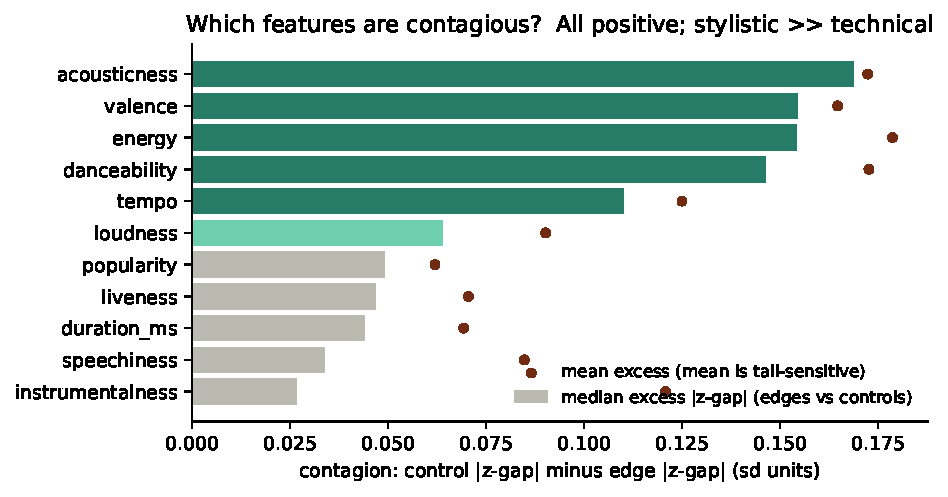
\includegraphics[width=0.9\textwidth]{feature_contagion_excess.pdf}
\caption{Contagion of musical characteristics: median (dark) and mean
(light) matched-control excess alignment per feature. Style
characteristics (acousticness, valence, energy, danceability) are
contagious; structural characteristics (instrumentalness, speechiness,
duration) are not.}
\label{fig:q4-features}
\end{figure}

\paragraph{Directional regression.}
Magnitude contagion does not imply \emph{directional} tracking. Fitting
$x_j^{f}=\beta_f x_i^{f}+\text{FE}+\varepsilon$ on the edges
(\cref{tab:q4-features}, columns 4--5), only \texttt{danceability}
($\beta=0.272$ versus $0.000$ on controls) and \texttt{valence}
($0.119$) show a clear ``influencer high $\Rightarrow$ follower high''
pull, while \texttt{energy}---strongly contagious in magnitude---has
$\beta\approx-0.03$. The divergence between $a_f$ and $\beta_f$ has a
natural reading: the average follower reports ${\sim}7.6$ influencers,
so a follower's coordinate is a mixture of many sources and random
dips; edges then show compressed \emph{distances} without linear
\emph{tracking}. Magnitude contagion and directional contagion are
different phenomena, and only danceability and valence pass both tests.

\subsection{Influence Strength versus Acoustic Trace}\label{subsec:q4-dose}

If reported influence were purely acoustic imitation, strongly
influential artists should leave stronger traces. The data show the
opposite. Binning edges by the influencer's outgoing Katz score of
Model~I (\cref{fig:q4-dose}, left), mean excess similarity declines
monotonically above the median: $0.040$ in the second Katz quintile
versus $0.028$ in the top quintile (Spearman
$\rho=-0.032$, $p<10^{-10}$ over edges). Highly influential artists are
cited \emph{beyond} what their sound predicts---a status component of
influence---whereas weaker influencers are cited precisely because
their sound is imitated. This complements Model~I, where edge counts
already separated reported prestige from network-transmitted influence.

\begin{figure}[htbp]
\centering
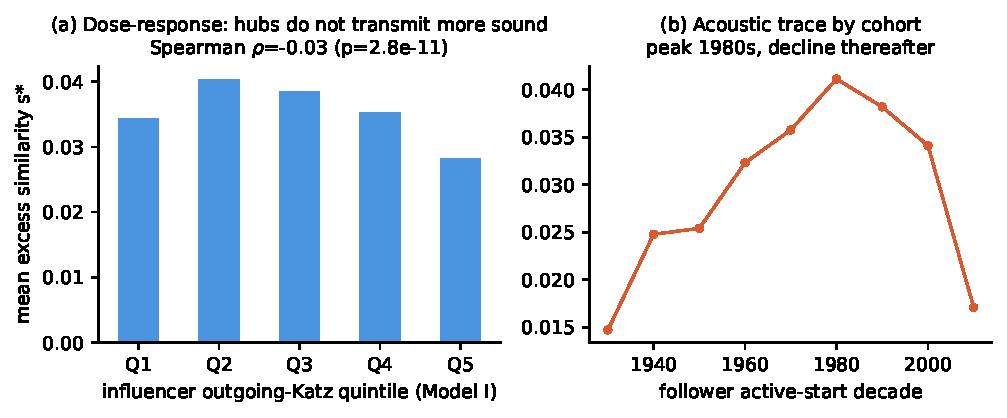
\includegraphics[width=0.95\textwidth]{dose_response_excess.pdf}
\caption{(a)~Mean excess similarity by influencer Katz quintile: the
acoustic trace \emph{weakens} for the most influential artists.
(b)~Mean excess similarity by follower active-start decade: the trace
rises to a 1980s peak ($0.041$) and falls sharply for the sparse 2010s
cohort ($n=798$).}
\label{fig:q4-dose}
\end{figure}

The decade curve (\cref{fig:q4-dose}, right) adds a temporal dimension
that connects to \cref{subsec:q3-inf-time}: the acoustic trace peaks for
followers starting in the 1980s ($0.041$) and collapses for the 2010s
cohort ($0.017$, $n=798$). Notably its peak lags the cross-genre flow
peak of \cref{subsec:q3-inf-time} (1960s) by two decades: the
\emph{breadth} of influence across genre boundaries narrowed first,
while the \emph{depth} of per-edge acoustic alignment kept rising into
the 1980s before falling---influence became narrower but more intense
before both declined.

\paragraph{Robustness and disclosure.}
The design inherits Assumption~A2 (active-start decade as the time
axis) and the cleaned edge table of section~4, including the $733$
time-reversed edges (A3); excluding them changes no conclusion because
the control construction does not depend on edge direction. The
\texttt{popularity} coordinate is retained for comparability with
Model~II, but its known within-year drift (section~5) makes its excess
($0.049$) hard to interpret, and it is excluded from the contagion
ranking. Raising the control count from $K=10$ to $K=25$ on a random
$4{,}000$-edge subsample changes $\bar{s}^{*}$ by $0.0004$. Two limitations bound the claims:
the data provide one acoustic snapshot per artist, so we cannot observe
change after the reported influence (hence ``consistent with'', not
``proves''), and influence not mediated by audio features (lyrics,
image, production practices) is invisible to this test.

\section{Model V: Temporal Dynamics}\label{sec:model-temporal}

\subsection{Revolutions as Punctuated Leaps (Task~5)}\label{subsec:t5-revolutions}

Task~5 asks which characteristics mark \emph{revolutions} (major leaps) in
musical evolution, and which artists are the corresponding revolutionaries.
We treat change as \emph{punctuated cultural evolution}: variants in a
population drift continuously~\cite{savage2019cultural}, but the rate of
change can spike in short windows~\cite{mauch2015evolution}. Operationally,
\emph{evolution} is gradual movement of the yearly feature state and slow
change of cross-genre influence shares, while a \emph{revolution} is a
short window in which the sonic leap size is anomalous relative to its
recent baseline, optionally reinforced by a simultaneous restructuring of
the influence network.

\paragraph{Sonic channel.}
Let \(\mathbf{x}(t)\in\mathbb{R}^{p}\) be the vector of the same \(p=11\)
Spotify features as Model~II, taken from \texttt{data\_by\_year} and
\(z\)-scored across years \(t\in[1930,2010]\). The sonic leap size is
\begin{equation}\label{eq:t5-E}
E(t)=\|\mathbf{x}(t)-\mathbf{x}(t-1)\|_2.
\end{equation}
Because early catalogue aggregates are thin and inflate a global threshold,
we score each \(E(t)\) by a rolling \(z\)-score against the preceding
12 leaps and call a \emph{sonic anomaly} when this local \(z\geq 2\) and
\(t\geq 1948\). The coordinates of \(\Delta\mathbf{x}(t)\) with largest
absolute share identify the driving characteristics of each leap. A Foote-style
past/future window novelty is retained as a robustness companion (same
qualitative peaks).

\paragraph{Network channel.}
We reuse the Model~III flow layer without redefining it: \(F(t)\)
is the genre-to-genre edge count matrix restricted to followers whose
active-start decade is \(t\), with cross-genre share \(c_{\mathrm{cross}}(t)\)
and Katz-weighted share \(c_K(t)\). Decade restructuring is summarised by
\begin{equation}\label{eq:t5-N}
N(t)
=\tfrac12\bigl|\Delta c_{\mathrm{cross}}(t)\bigr|
+\tfrac12\bigl|\Delta c_K(t)\bigr|
+\tfrac14\,\tau(t),
\end{equation}
where \(\tau(t)\) is the \(\ell_1\) turnover of genre shares of outgoing
Katz mass \(K_g(t)\) among artists starting in decade \(t\). Decades with
\(z\)-scored \(N(t)\) above \(0.75\) are network anomalies. This keeps the
same follower-start decade clock as Assumption~A2 and as \(F(t)\), \(c_K(t)\)
in \cref{subsec:q3-inf-time}.

\paragraph{Dual-channel labels.}
A decade is \emph{strong} if it contains at least one sonic anomaly and is a
network anomaly; \emph{weak} if exactly one channel fires; otherwise
\emph{evolution}. Empirically the only strong decade is the 1970s (sonic
peak in 1976; sharp drop in \(c_{\mathrm{cross}}\) and \(c_K\) after the
1950--60s cross-genre high). The 1950s are a network-only weak signal:
\(c_K(t)\) peaks near \(0.53\) while local sonic \(z\) stays below the
cutoff---an influence-structure rewiring (rock \& roll / R\&B export) that
is louder in \(F(t)\) than in yearly mean features. Pre-1948 spikes in raw
\(E(t)\) are plotted but not labelled revolutions (composition caution).

\begin{figure}[t]
\centering
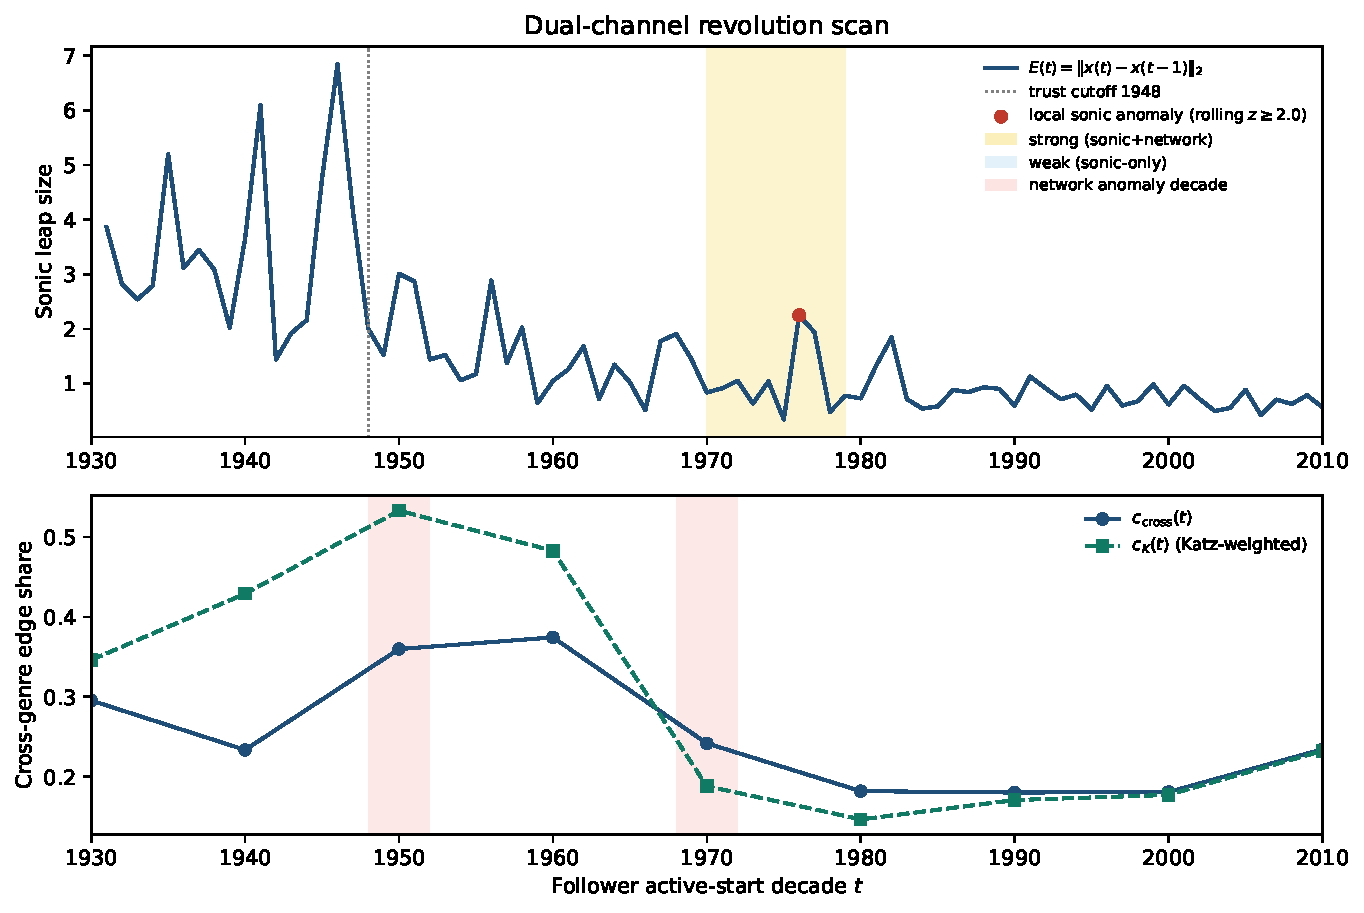
\includegraphics[width=0.68\textwidth]{fig_t5_dual_channel_revolutions.pdf}
\caption{Dual-channel scan: sonic leap \(E(t)\) (top; local \(z\geq 2\),
\(t\geq 1948\)) and network shares \(c_{\mathrm{cross}}(t)\), \(c_K(t)\)
(bottom). Gold = strong 1970s; network-only weak = 1950s.}
\label{fig:t5-dual}
\end{figure}

\paragraph{Characteristics that signify leaps.}
In the strong 1970s window the dominant driver of \(\Delta\mathbf{x}\) is
\texttt{liveness}, followed by \texttt{duration\_ms} and \texttt{tempo}:
the leap is a production/performance shift rather than a single
``genre birth'' coordinate. Network-side, the signifying quantity is the
collapse of cross-genre share after its mid-century plateau
(\(c_{\mathrm{cross}}\approx 0.36\)--\(0.37\) in 1950--60 down to
\(\approx 0.18\) by 1980--2000), i.e.\ influence re-concentrates inside
genres even while sonic drift continues slowly.

\paragraph{Revolutionaries.}
Within a flagged decade \(d\) we score artists who began no later than \(d\)
by a blend of outgoing Katz \(K_i\), the number of followers whose
active-start lies in \(\{d,d+10\}\), and the alignment of their feature
displacement from the previous-decade mean of \(\mathbf{x}(t)\) with the
window's mean sonic direction \(\Delta\mathbf{x}\). This prefers transmitters
who move \emph{with} the leap and are followed afterward, not artists who
merely correlate with the industry average. Top names in the 1950s weak
window include Chuck Berry, Little Richard and James Brown; in the 1970s
strong window, Bob Dylan, The Rolling Stones and Jimi Hendrix
(\cref{tab:t5-revs}).

\begin{table}[htbp]
\centering
\caption{Top revolutionaries by dual-channel window (score blend of \(K_i\),
followers in \(\{d,d+10\}\), and sonic alignment).}
\label{tab:t5-revs}
\small
\begin{tabular}{cllll}
\toprule
Decade & Label & Artist & Genre & \(K_i\) rank signal \\
\midrule
1950s & weak (network) & Chuck Berry & Pop/Rock & high \(K_i\), many 1950/60 followers \\
1950s & weak (network) & Little Richard & Pop/Rock & high alignment + followers \\
1950s & weak (network) & James Brown & R\&B & cross-genre transmitter \\
1970s & strong & Bob Dylan & Pop/Rock & top score in window \\
1970s & strong & The Rolling Stones & Pop/Rock & high \(K_i\) + followers \\
1970s & strong & Jimi Hendrix & Pop/Rock & strong sonic alignment \\
\bottomrule
\end{tabular}
\end{table}

\paragraph{Limits.}
\texttt{data\_by\_year} is a Spotify-era mean catalogue, not a probability
sample of all music; early \(E(t)\) is composition-sensitive. Influence edges
are reported relations, and decade \(t\) indexes follower start years, not
event dates. Detected leaps are statistical rate spikes, offered as
candidates for historical interpretation rather than causal claims.

% T6 is included from main.tex via model4_t6.tex (subsection under this Model V).
% TODO (T7): pre/post-1995 era slicing; internet effect on network + features.


\subsection{The Jazz Influence Process over Time (Task~6)}\label{subsec:t6-jazz}

Task~6 asks for the influence process of musical evolution over time in one genre, for indicators
that reveal the dynamic influencers, and for an explanation of how the genre and its artists
changed. We study jazz. The choice continues \cref{subsec:q1-jazz}: the Jazz-induced subnetwork
there (384 artists, 1,769 edges) is the genre subnetwork examined in Model~I, and it spans the
whole record. It also gives the revolution windows of T5 (\cref{subsec:t5-revolutions}) a
genre-level test: the question is not only whether a decade is a revolution in the all-genre
catalogue, but which jazz artists moved, and whether their followers moved with them.

\paragraph{A release-year timeline.}
We use the same 42,770 edges as Model~I under Assumption~A3, including the 733 time-order
reversals. 406 artists carry the Jazz label; 384 of them form the both-endpoints-jazz
subnetwork of \cref{subsec:q1-jazz}. The Spotify files contain 8,000 jazz songs by
404 of these artists; 285 artists have at least three songs and can be given
a stable feature vector. Three clocks are kept separate: a song's release year \(y\), an artist's
active-start decade \(t_i\), and a follower's active-start decade (the cohort clock of
\cref{subsec:q1-cohorts}). The first describes the genre's sound, the second places an artist's
generation, and the third is used to validate transmission.

Model~II represents an artist by eleven Spotify coordinates (\cref{sec:model-similarity}); we use
its nine \emph{sound} coordinates, dropping \texttt{liveness} and \texttt{popularity}. Liveness
separates live from studio recordings --- a \(k\)-means run that includes it sets apart a
589-song cluster almost entirely by liveness ($+4.7$ standard deviations) --- and
popularity is not a property of the sound. All coordinates are \(z\)-scored across the artists of
\texttt{data\_by\_artist.csv}. This is a deliberate difference from T5, which uses all eleven
yearly aggregates and finds liveness the dominant 1970s driver; the robustness paragraph below
shows that adding liveness back changes the indicator rankings only marginally.

For each year with at least 20 jazz songs we compute the mean \(z\)-vector
\(\mathbf{x}_J(y)\), smooth it with a centred three-year window, and interpolate between years.
This leaves a reliable series from 1936 to 2002; earlier and later years are too sparse
for a yearly curve, and the 2010s (22 songs) are excluded from the decade summaries. A principal
component analysis of the yearly centroids gives PC1 59.3\% (acoustic and short recordings at
the positive end, long and electric ones at the negative end; loadings duration $-0.79$, acousticness $+0.52$, energy $-0.24$) and PC2
16.8\% (loadings instrumentalness $+0.58$, energy $+0.48$, valence $+0.42$). \cref{fig:t6-timeline} shows the decade trajectory and the
standardized decade centroids.

\begin{figure}[htbp]
\centering
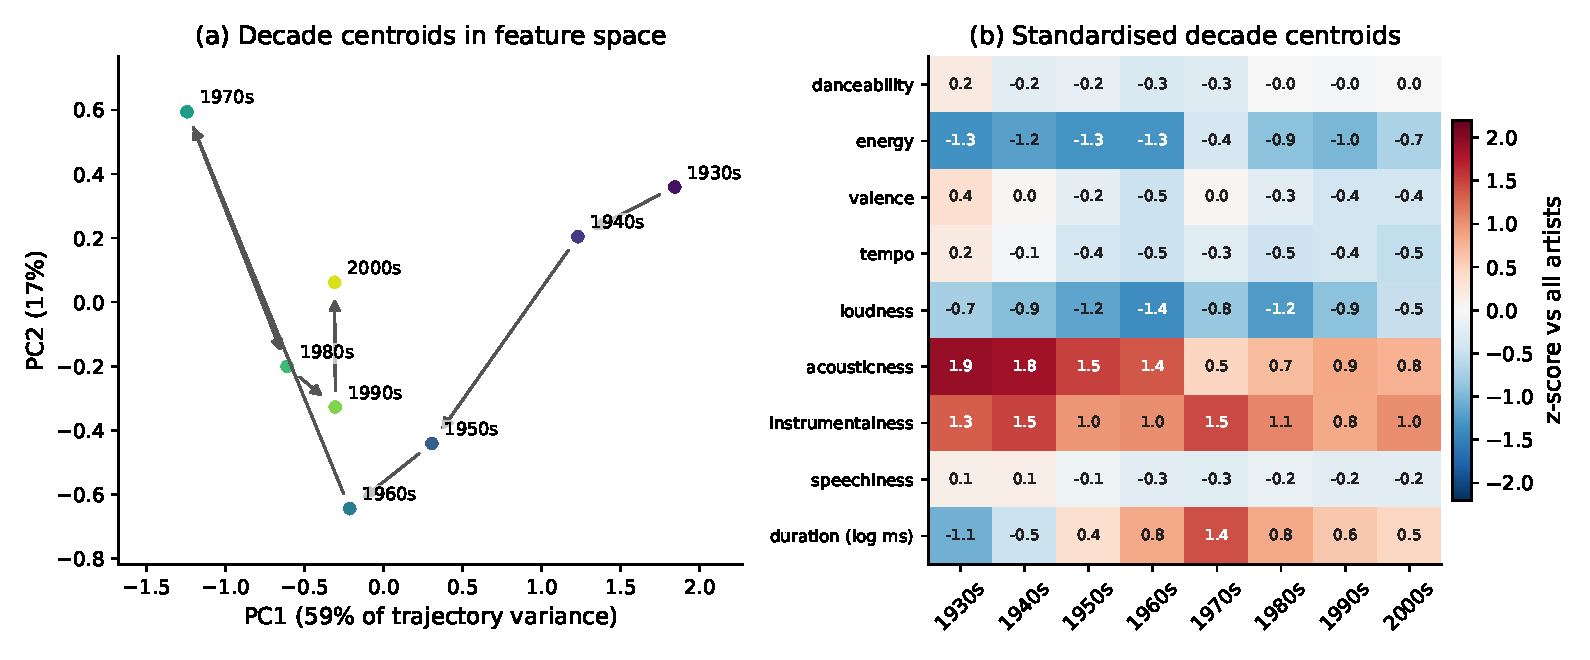
\includegraphics[width=\textwidth]{fig_t6_timeline.pdf}
\caption{Jazz sonic timeline. (a) Decade centroids in the first two principal components of the
yearly release-year centroids; arrows follow the decades. (b) Standardized decade centroids of the
nine sound features.}
\label{fig:t6-timeline}
\end{figure}

The trajectory is a loop. The 1930s centroid is the most acoustic and the shortest of the series
(acousticness 0.91, duration 3.0 min, tempo 124 BPM, valence
0.62); the 1950s--60s lengthen and darken; the 1970s is the most electric, highest-energy
and longest decade (acousticness 0.48, energy 0.51, duration 6.7 min); and
the 1980s--2000s recover part way towards an acoustic sound (0.55, 0.60,
0.57) without returning to the 1930s values.

\paragraph{Four jazz-specific episodes.}
The speed \(\|\mathbf{x}_J(y+2)-\mathbf{x}_J(y-2)\|\) has four well-separated local maxima, at
1949, 1954, 1969 and 1980 (\cref{fig:t6-episodes}). Their feature decompositions separate a stylistic break, a
format change, an electric turn and a crossover reversal:
\begin{itemize}[leftmargin=1.2em,itemsep=0.15em]
\item 1949: duration $-1.28$, loudness $-1.07$, energy $-1.00$ --- the small-group bebop break with swing;
\item 1954: duration $+1.58$, instrumentalness $-0.43$, valence $-0.18$ --- consistent with the LP replacing the 78-rpm single;
\item 1969: duration $+0.76$, energy $+0.56$, acousticness $-0.55$ --- fusion and electric instruments;
\item 1980: speechiness $+0.59$, loudness $-0.51$, valence $-0.51$ --- crossover, smooth jazz and the start of the acoustic revival.
\end{itemize}
The 1969 episode is the jazz face of T5's strong 1970s window (\cref{fig:t5-dual}), and the 1954
format shift corresponds to T5's network-only weak 1950s window. T5 reaches the 1970s through
liveness (a production shift); the jazz-only space reaches it through acousticness, energy and
duration (a style shift). The two readings are complementary.

\begin{figure}[htbp]
\centering
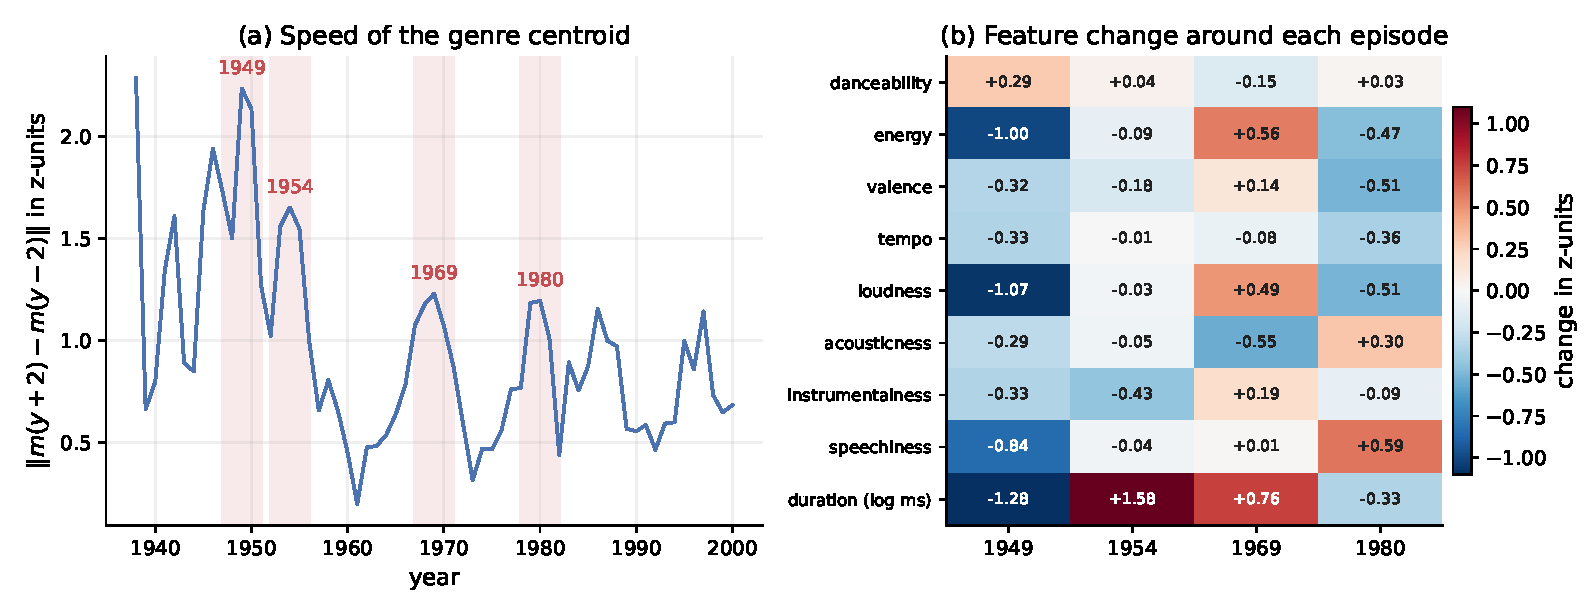
\includegraphics[width=\textwidth]{fig_t6_episodes.pdf}
\caption{Four jazz-specific episodes. (a) Speed of the jazz centroid; shaded bands mark the
episodes. (b) Change in each feature around each episode, $\mathbf{x}_J(y+2)-\mathbf{x}_J(y-2)$ in
\(z\)-units.}
\label{fig:t6-episodes}
\end{figure}

\paragraph{Indicators of dynamic influence.}
For artist \(i\) with \(n_i\ge3\) songs, let
\begin{equation}\label{eq:t6-r}
r_i=\frac{1}{n_i}\sum_{s\in i}\bigl(\tilde{\mathbf{x}}_s-\mathbf{x}_J(y_s)\bigr)
\end{equation}
be the \emph{time-adjusted deviation}: the average of the song vectors, each centred on the jazz
sound of its release year. The four indicators are:
\begin{align}
N_i&=\|r_i\|_\Sigma, \label{eq:t6-N}\\
A_i&=\cos(r_i,\Delta_i),\qquad \Delta_i=\mathbf{x}_J(t_i+10)-\mathbf{x}_J(t_i),
\label{eq:t6-A}\\
H_i&=\frac{1}{n_i^H}\sum_{j:\,i\to j,\ t_j>t_i}\cos(r_j,r_i),\qquad
H_i^*=H_i\,\frac{n_i^H}{n_i^H+3}, \label{eq:t6-H}
\end{align}
where \(N_i\) is originality (Mahalanobis length), \(A_i\) is anticipation (does the artist's
deviation point where the genre went over the next decade?), and \(H_i^*\) is transmission (did the
followers who name \(i\) move in \(i\)'s direction?), shrunk for small follower counts. Reach is
measured by \(K_i\), the within-jazz Katz score of \cref{subsec:q1-jazz}, and by \(B_i\), the number
of non-jazz followers; the Jazz$\to$Pop/Rock block alone contains 409 edges
(\cref{subsec:q3-inf-time}). The sonic indicators are defined for 283 artists; 175 have
a usable transmission score and 59 have at least five jazz followers.

\paragraph{Validation.}
There are 937 jazz$\to$jazz pairs with a later follower and at least three songs for both
artists. The mean alignment is 0.164. A within-decade permutation null (2{,}000 draws)
gives 0.024 \(\pm\) 0.030, so $p<0.001$; the bootstrap 95\% interval is
\([0.105,0.222]\). 56.4\% of the real pairs are positive against
51.2\% in the null. The effect is modest but real: reported influence is visible as a
small average movement of the follower's music in the influencer's direction. This complements the
matched-control similarity test of Task~4, which asks whether followers are closer to their
influencers than to controls; the present test asks whether they move \emph{towards} the
influencer's deviation from their own era.

The indicators are not redundant: \(N\)--\(A\) -0.02, \(N\)--\(K\) -0.37,
\(A\)--\(K\) +0.11, \(H^*\)--\(K\) +0.25. Originality is negatively related to citation
(-0.35 with future followers), anticipation is nearly independent of it (+0.09), and
transmission is the closest to future citation (+0.29). The most novel artists are not the
most cited, and being ahead is not the same as being central.

\paragraph{Dynamic influencers.}
We rank artists by \(S_i=z(A_i)+z(H_i^*)\), the equal-weight sum of the two standardized sonic
indicators, among the 59 artists with at least five jazz followers. Ranks are stable to
the weights (Spearman 0.910--0.979 for \(A\) weights 0.3--0.7) and to the transmission shrinkage
(raw and shrunk \(H\) correlate at 0.993). \cref{tab:t6-top} gives the top twelve;
\cref{fig:t6-influencers} maps anticipation against transmission.

\begin{table}[htbp]
\centering
\small
\caption{Top twelve dynamic influencers. \(N\) originality, \(A\) anticipation, \(H^*\)
transmission, ``Followers'' the number of usable jazz followers, \(K\) within-jazz Katz, \(B\)
non-jazz followers.}
\label{tab:t6-top}
\begin{tabular}{rlccccccc}
\toprule
\# & Artist & Start & \(N\) & \(A\) & \(H^*\) & Followers & \(K\) & \(B\) \\
\midrule
1 & Dave Brubeck & 1940s & 1.13 & +0.61 & +0.62 & 8 & 2.13 & 6 \\
2 & George Duke & 1960s & 1.62 & +0.36 & +0.66 & 5 & 1.69 & 10 \\
3 & Tal Farlow & 1940s & 2.46 & +0.92 & +0.38 & 8 & 3.03 & 2 \\
4 & Grover Washington, Jr. & 1960s & 1.19 & +0.23 & +0.70 & 8 & 2.32 & 1 \\
5 & David Sanborn & 1960s & 1.43 & +0.76 & +0.30 & 5 & 1.76 & 0 \\
6 & Bob James & 1960s & 1.76 & +0.30 & +0.50 & 6 & 1.77 & 2 \\
7 & Barney Kessel & 1940s & 3.38 & +0.69 & +0.23 & 6 & 4.81 & 2 \\
8 & Erroll Garner & 1940s & 2.18 & +0.74 & +0.20 & 11 & 4.52 & 4 \\
9 & Nat King Cole & 1930s & 2.31 & +0.54 & +0.27 & 11 & 5.07 & 52 \\
10 & Horace Silver & 1950s & 1.64 & +0.53 & +0.26 & 11 & 5.76 & 5 \\
11 & Oscar Peterson & 1940s & 2.44 & +0.79 & +0.12 & 14 & 4.66 & 4 \\
12 & Clifford Brown & 1950s & 1.42 & +0.69 & +0.15 & 6 & 3.13 & 0 \\
\bottomrule
\end{tabular}
\end{table}

\begin{figure}[htbp]
\centering
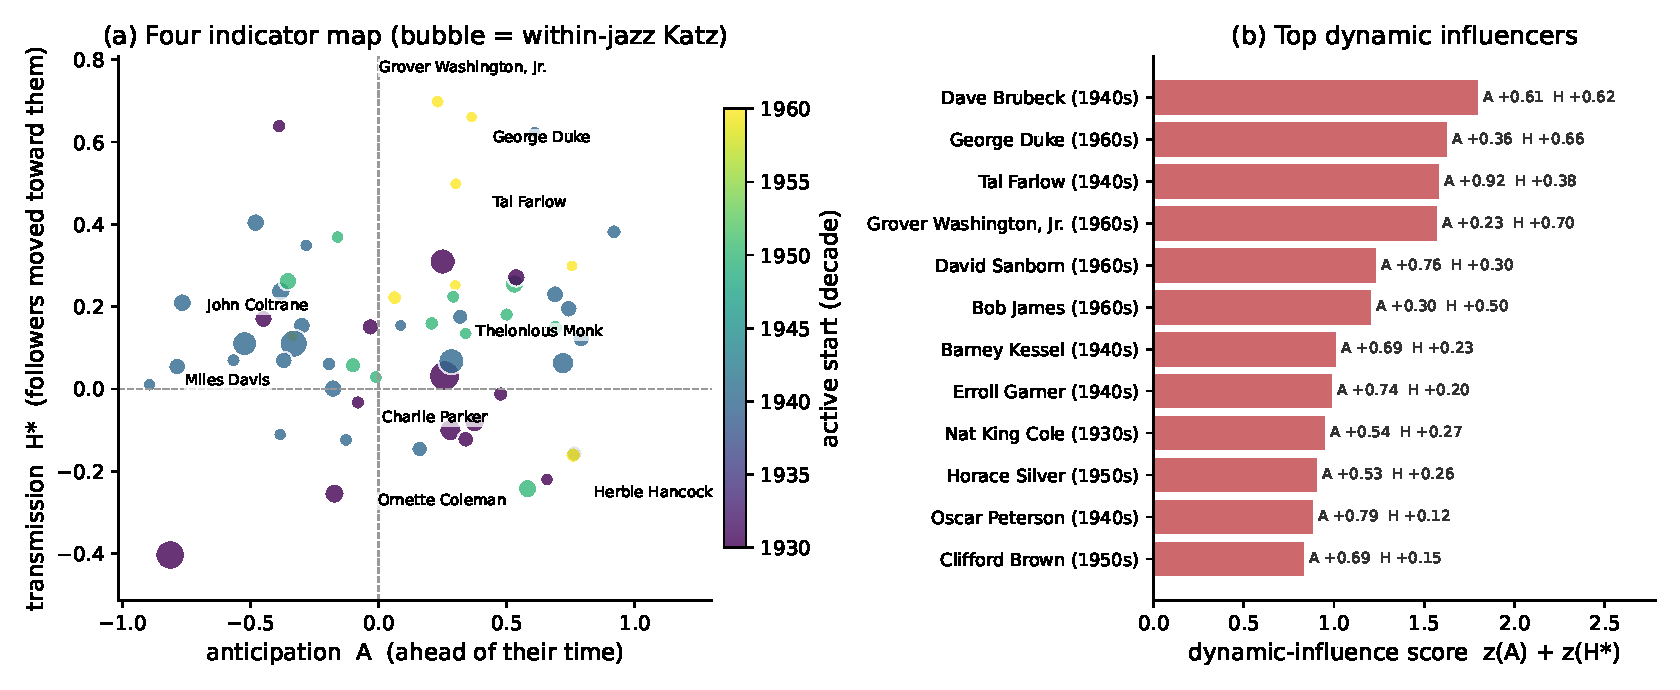
\includegraphics[width=\textwidth]{fig_t6_influencers.pdf}
\caption{(a) Anticipation against transmission for artists with at least five jazz followers;
bubble area is within-jazz Katz and colour is the active-start decade. (b) The top twelve by
\(S=z(A)+z(H^*)\), annotated with the two component scores.}
\label{fig:t6-influencers}
\end{figure}

\paragraph{Four roles.}
The \emph{canon} (high \(K\)) is Charlie Parker (17.2), Lester Young (15.5), Miles
Davis (13.9), Dizzy Gillespie, Thelonious Monk and John Coltrane (10.8). Their
anticipation is mixed and often negative, because they define the centre of their generation. The
\emph{catalysts} have high \(A\) and high \(H^*\): Dave Brubeck (+0.61/+0.62), George
Duke, Tal Farlow (+0.92), Grover Washington, Jr., David Sanborn and Bob James. The
\emph{prophets} are ahead but not copied: Duke Jordan, Shelly Manne, Jimmy Giuffre and John Lewis,
with Herbie Hancock (+0.76/-0.16), Lee Morgan and Andrew Hill in the 1960s
generation. The \emph{bridges} export influence beyond jazz: Miles Davis (77 non-jazz
followers), Nat King Cole (52), John Coltrane (52), Quincy Jones (25)
and Sun Ra (24).

\paragraph{How jazz changed.}
The swing baseline is acoustic and short (1930s: 0.91, 3.0 min, 124
BPM); Lester Young is the pure canon type ($K=15.5$, $A=-0.81$), and Cab Calloway is a
bridge (23 non-jazz followers). The 1949 bebop break
is visible in the cohort, not in Parker's distance from it: Parker has the highest within-jazz Katz
(17.2) but only $A=+0.26$ and $H^*=+0.03$; Bud Powell ($A=+0.72$) and
Gillespie ($H^*=+0.31$) carry more of the directional signal. The 1950s add the LP and
hard bop: Brubeck (+0.61/+0.62), Farlow ($A=+0.92$), Horace Silver
($A=+0.53$/$H^*=+0.26$) and Clifford Brown ($A=+0.69$). The late 1950s--60s
separate the canon from the avant-garde: Coltrane and Miles remain central ($K=10.8$
and 13.9) with negative anticipation, while Ornette Coleman
($A=+0.58$/$H^*=-0.24$, 16 non-jazz followers), Cecil Taylor
($A=+0.81$, $K=1.7$), Herbie Hancock ($A=+0.76$/$H^*=-0.16$) and
Andrew Hill ($A=+0.70$/$H^*=-0.31$) are ahead of the centre. The 1970s is fusion:
Hancock, Tony Williams ($A=+0.73$), John McLaughlin ($A=+0.38$/$H^*=+0.48$,
5 non-jazz followers) and Weather Report (10 non-jazz followers), with
Miles as the boundary bridge. The 1980s--2000s turn to crossover: George Duke
(+0.36/+0.66), Grover Washington, Jr. (+0.23/+0.70), Bob James
(+0.30/+0.50) and David Sanborn (+0.76/+0.30), with Wynton Marsalis
($A=+0.31$) marking the neoclassical reaction but having no usable jazz follower in this
edge set.

Across the period the influence process has two mechanisms. \emph{Canonical transmission}
reproduces the centre: the most cited artists define what the next generation sounds like, which
shows up as high \(K\) with low \(A\) and \(H^*\). \emph{Catalytic transmission} moves the centre: an
artist's deviation points where the genre goes and the followers move towards it, which shows up as
high \(A\) and \(H^*\). The largest movements occur when the second mechanism meets an opening that
is not itself musical --- the LP in the 1950s, electric instruments and amplification in the late
1960s, and multitrack production in the 1980s. This is also where the social and technological
dimension of the problem enters the network: it enters as a change of recording format and
production that shifts the feature centroid before the influence network catches up.

\paragraph{Limits and robustness.}
Only 285 of the 406 jazz artists have at least three songs, 175 have a usable
transmission score, and 59 have at least five followers; the ranking is therefore
descriptive rather than definitive. The 2010s (22 songs) are excluded; the 1920s contain only 9.
Active-start is a decade, it comes from AllMusic while the features come from Spotify, and a
song's year is its release year, not its composition year. Career averages are replaced by
song-level residuals, but the genre label remains coarse: ``Jazz'' covers swing, bebop, free jazz
and smooth jazz. Leave-one-out centroids change the originality and anticipation rankings by
Spearman 0.996 and 0.999; adding liveness gives 0.965 and 0.993; a five-year
anticipation horizon gives 0.766. The transmission test controls for decade composition but not
for shared scene or label, and it is an association between reported influence and sonic
direction, not a causal effect.


\section{Validation and Sensitivity Analysis}\label{sec:validation}
% TODO: validation checks; sensitivity table over key parameters; limitations.

\section{Strengths, Weaknesses and Conclusion}\label{sec:conclusion}
% TODO: strengths; weaknesses; conclusion per task.

%------------------------------------------------------------------------------
% 4. ONE-PAGE DOCUMENT TO THE ICM SOCIETY — must fit on ONE page.
%    Cover: (i) value of our approach; (ii) how richer data would change our
%    work; (iii) recommendations for further study of music and culture.
%------------------------------------------------------------------------------
\newpage
\section*{A Document to the ICM Society}
\addcontentsline{toc}{section}{A Document to the ICM Society}
\label{sec:memo}
\noindent\begin{tabular}{@{}ll@{}}
  \textbf{To:}      & The Integrative Collective Music (ICM) Society \\
  \textbf{From:}    & Team 123090276/123090452/123090773 \\
  \textbf{Subject:} & The value of network-based measures of musical influence \\
  \textbf{Date:}    & November 29, 2026 \\
\end{tabular}
% TODO: memo body (keep within one page).

%------------------------------------------------------------------------------
% 5. REFERENCES — cite every external source of data, ideas, figures and code.
%    Do NOT invent references.
%------------------------------------------------------------------------------
\newpage
\begin{thebibliography}{99}
\bibitem{allmusic} AllMusic. \emph{Music data scraped from AllMusic.com}, 2021.
\bibitem{spotify} Spotify. \emph{Spotify Web API audio features}, 2021.
\bibitem{mauch2015evolution}
  M.~Mauch, R.~M.~MacCallum, M.~Levy and A.~M.~Leroi.
  The evolution of popular music: USA 1960--2010.
  \emph{Royal Society Open Science}, 2(5):150081, 2015.
\bibitem{savage2019cultural}
  P.~E.~Savage.
  Cultural evolution of music.
  \emph{Humanities and Social Sciences Communications}, 5:16, 2019.
% ... add your actual sources here.
\end{thebibliography}

%------------------------------------------------------------------------------
% 6. CONTRIBUTION STATEMENT — final page, NOT counted in the 25-page limit.
%------------------------------------------------------------------------------
\newpage
\section*{Contribution Statement}
% TODO: who did what, ordered by ascending student ID; note the code README.
\begin{itemize}
  \item \textbf{Li Peixuan (123090276):} ...
  \item \textbf{Qian Chenghao (123090452):} ...
  \item \textbf{Yu Zihan (123090773):} ...
\end{itemize}

\end{document}
